\documentclass[11pt,a4paper]{article}
\usepackage[utf8]{inputenc}
\usepackage{amsmath}
\usepackage{amsfonts}
\usepackage{amssymb}

\usepackage{todonotes}
\usepackage{todoextend}


\usepackage{color}
\usepackage{listings}
\renewcommand\lstlistingname{Code Segment}
\definecolor{dkgreen}{rgb}{0,0.6,0}
\definecolor{gray}{rgb}{0.9,0.9,0.9}
\definecolor{mauve}{rgb}{1,0.4,0}
\lstset{frame=none,
  backgroundcolor=\color{gray},
  escapeinside={\%*}{*)},
  language=R,
  aboveskip=3mm,
  belowskip=3mm,
  showstringspaces=false,
  columns=flexible,
  basicstyle={\small\ttfamily},
  numbers=left,
  numberstyle=\tiny\color{black},
  keywordstyle=\color{blue},
  commentstyle=\color{dkgreen},
  stringstyle=\color{mauve},
  breaklines=true,
  breakatwhitespace=true,
  tabsize=3,
  captionpos=b,
  xleftmargin=.25in,
  xrightmargin=.25in
}

\usepackage{multirow}

\usepackage{graphicx}
\usepackage{epstopdf} % for eps file

\usepackage{fullpage} % utilize paper space :)

\usepackage{float} % for use of [H] in figure alignment
\usepackage{subcaption} % for use of subfigures
\usepackage{tikz}

\usepackage{hyperref}
\hypersetup{
pdfborder = {0 0 0}
}



\setlength{\parindent}{0pt}
\setlength{\parskip}{0.5\baselineskip}%

\DeclareMathSizes{12}{14}{10}{10} % increase math font size

\begin{document}

\title{K-NN and Trees\\Statistical Machine Learning\\{\large\emph{Group 3}}}
\author{Nikolaj Iversen and Lukas Schwartz}
\date{June 9$^{th}$, 2015}
\maketitle

\vfill
\begin{center}
\includegraphics[width=0.7\textwidth]{graphics/digit_example}
\end{center}

\newpage


\section*{Abstract}



\section*{Acknowledgement}
This piece is written as a report by Nikolaj Iversen and Lukas Schwartz.
...


\newpage

\tableofcontents
\listoffigures
\listoftables

\newpage


\section{Introduction}

The classification of handwritten characters is used in a wide range of products to day.
Hence, this report goes in depth with how the numbers from zero to nine can be classified using machine learning algorithms.

The data set consists of a set of handwritten characters from zero to nine.
These were constructed by the students enrolled in the course Statistical Machine learning (RM-SML-E1) in 2015 at the University of Southern Denmark (SDU).
The characters were written in boxes of $0.55 \times 0.55 \textit{ cm}$ on a sheet with $20 \times 20$ boxes for each character.
The set used in this report is the 100DPI dataset.
Each number is hence stored as a $20 \times 20 \textit{ pixel}$ matrix containing the handwritten character.

The methods used for classification are K-Nearest Neighbours and Decision Trees.
This is to compare a method of lazy supervised learning against a method of supervised learning.
Furthermore a set of different ways to pre-process the data is explored.
Finally the two methods are compared with each at the best parameters and preprocessing settings.

The goal is to tests the handwritten digits from 20 people enrolled in the course.
The first test is where all people are mixed together, everybody contributing 90\% of their data to the training set and 10\% to the test set.
This is considered the easy problem as special ways of writing a digit will be represented in the training data.

Another test is to use 19 people's digits as training data and use the last person to test.
This is considered the hard problem.

To test the performance of the classification methods a simplified problem has been constructed.
It takes training data from a single person, Lukas Schwartz, which is referred to as Group 3 member 2 (G3M2).
By splitting the data 90\% for training and 10\% for testing
360 digits from each class as training data and 40 digits was used.
Testing each parameter with the simplified problem means the parameters could be tested in less time than if using the entire data set.

\newpage

\section{Preprocessing}
\section{Introduction}

The classification of handwritten characters is used in a wide range of products to day.
Hence, this report goes in depth with how the numbers from zero to nine can be classified using machine learning algorithms.

The data set consists of a set of handwritten characters from zero to nine.
These were constructed by the students enrolled in the course Statistical Machine learning (RM-SML-E1) in 2015 at the University of Southern Denmark (SDU).
The characters were written in boxes of $0.55 \times 0.55 \textit{ cm}$ on a sheet with $20 \times 20$ boxes for each character.
The set used in this report is the 100DPI dataset.
Each number is hence stored as a $20 \times 20 \textit{ pixel}$ matrix containing the handwritten character.

The methods used for classification are K-Nearest Neighbours and Decision Trees.
This is to compare a method of lazy supervised learning against a method of supervised learning.
Furthermore a set of different ways to pre-process the data is explored.
Finally the two methods are compared with each at the best parameters and preprocessing settings.

The goal is to tests the handwritten digits from 20 people enrolled in the course.
The first test is where all people are mixed together, everybody contributing 90\% of their data to the training set and 10\% to the test set.
This is considered the easy problem as special ways of writing a digit will be represented in the training data.

Another test is to use 19 people's digits as training data and use the last person to test.
This is considered the hard problem.

To test the performance of the classification methods a simplified problem has been constructed.
It takes training data from a single person, Lukas Schwartz, which is referred to as Group 3 member 2 (G3M2).
By splitting the data 90\% for training and 10\% for testing
360 digits from each class as training data and 40 digits was used.
Testing each parameter with the simplified problem means the parameters could be tested in less time than if using the entire data set.


\subsection{Smoothing}
\label{sec:smoothing}
The process of smoothing involves applying a kernel to an image using convolution.
Smoothing is applied to an image in order to reduce the noise in the image such that only the important features are left in the data.
A wide range of kernels can be used for smoothing, but in this report only the Gaussian kernel is considered.
Furthermore, the kernels considered here all have a sum of one, such that the brightness of the image is unchanged.

When applying a smoothing filer, the neighbouring pixels to the smoothed are added a contribution from the smoothed.
The process of smoothing hence widens the digits, as seen in figure \ref{fig:effect_smooth}, and this should give a better chance of two characters overlapping.
The danger is that too much smoothing blurs the whole image and hence remove the features in the data that is used to compare and identify the characters.

\begin{figure}[H]
\centering
	\begin{subfigure}[b]{0.2\textwidth}
	\includegraphics[width=\textwidth]{graphics/smooth_none}
	\caption{Raw image.}
	\end{subfigure}
	\qquad
	\begin{subfigure}[b]{0.2\textwidth}
         \includegraphics[width=\textwidth]{graphics/smooth_05_5}
         \caption{\(\sigma = 0.5\).}
	\end{subfigure}
	\qquad
	\begin{subfigure}[b]{0.2\textwidth}
         \includegraphics[width=\textwidth]{graphics/smooth_1_5}
         \caption{\(\sigma = 1\).}
	\end{subfigure}
	\qquad
	\begin{subfigure}[b]{0.2\textwidth}
         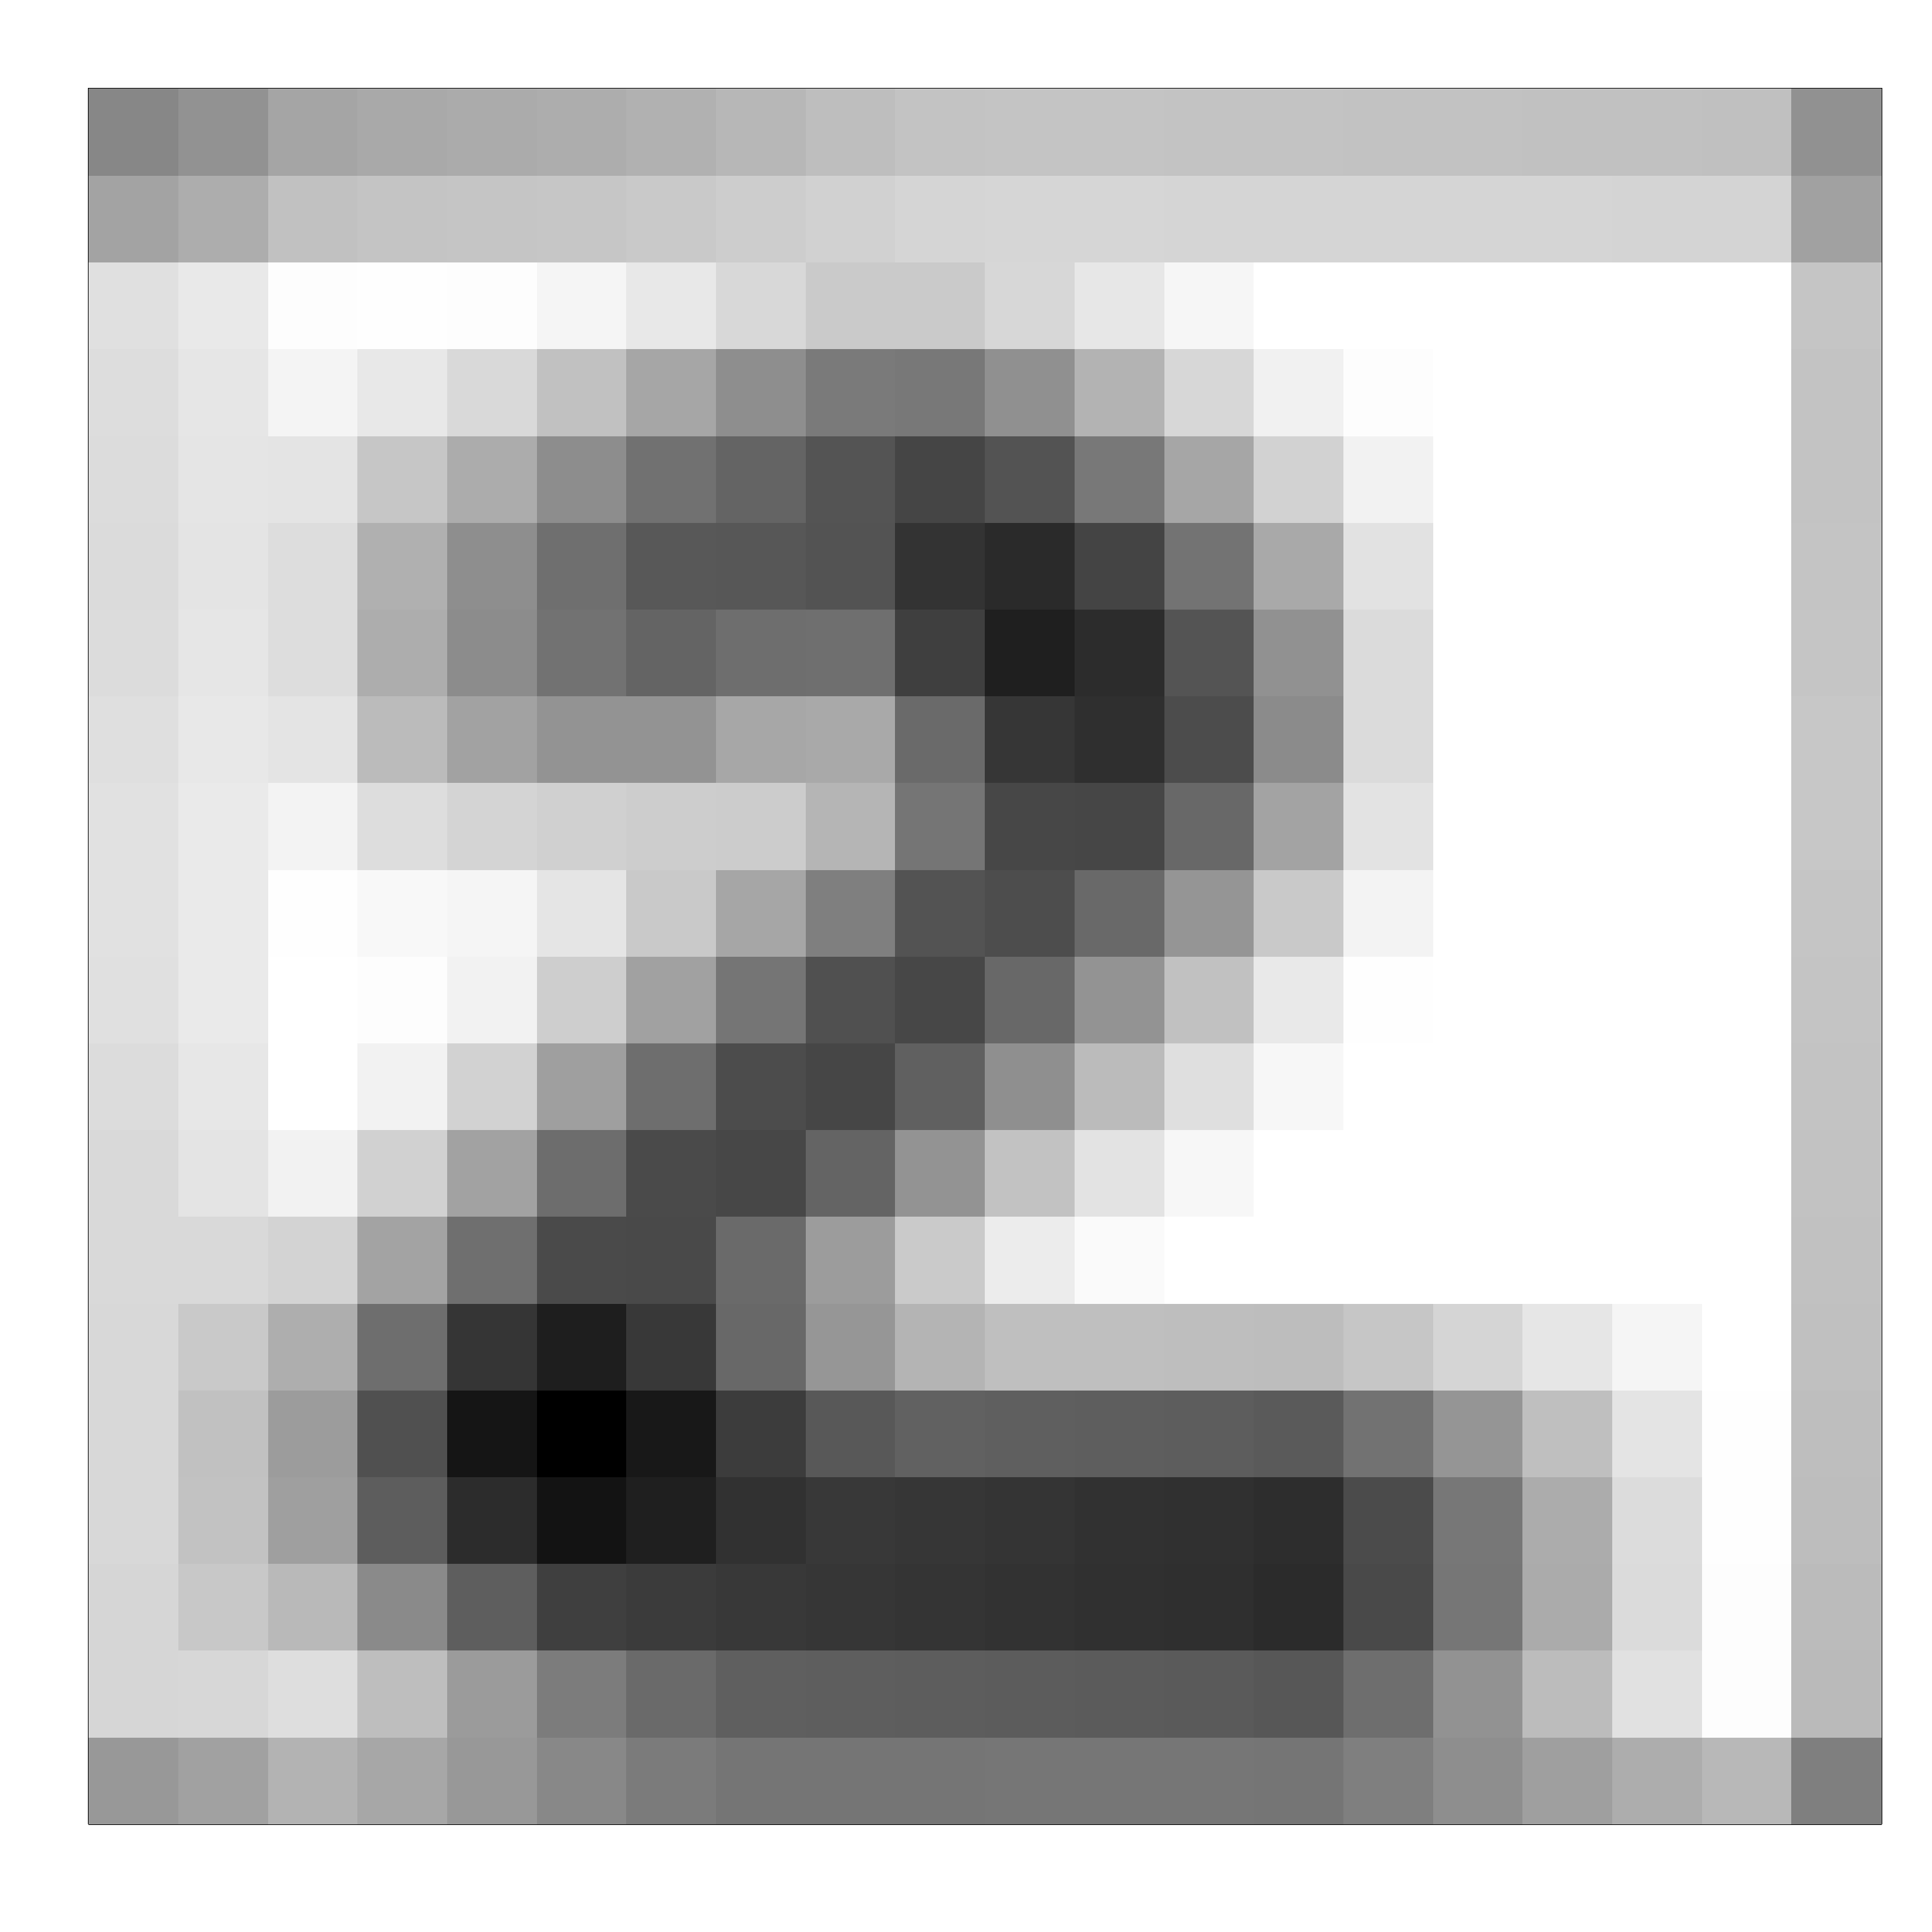
\includegraphics[width=\textwidth]{graphics/smooth_2_5}
         \caption{\(\sigma = 2\).}
	\end{subfigure}
\caption{Illustration of Gaussian smoothing. All kernels are 5x5.}
\label{fig:effect_smooth}
\end{figure}

A Gaussian distribution (also referred to as a normal distribution) is a naturally occurring distribution which is found when a random result occurs around a mean. 
The $\sigma$ signifies the deviation of the distribution. 
The 2D equation of a Gaussian distribution is shown in equation \ref{eq:gauss}. 

\begin{equation}
G(x,y) = \frac{1}{2\pi \sigma^2} e^{- \frac{x^2+y^2}{2\sigma^2}} \label{eq:gauss}
\end{equation}

Using the Gaussian filter to smooth an image will weigh the distance to the pixel.
A small $\sigma$ will make a small deviation and thus heavily weigh the center pixel.
The Gaussian filter is the one applied in figure \ref{fig:effect_smooth}.

%Applying a smoothing function can give the image an advantage when using the nearest neighbour analysis.

%The results of the filtering methods were also compared to the raw image with 100, 200 and 300 DPI.
%These results are compared with an averaging filter (avg) which takes the average of the four neighbouring pixels and a Gaussian filter (G) with different values for sigma.
%These tests were done 10 times, using cross validation, and the mean of each success rate is plotted in figure \ref{fig:smooth}. 
%Since the variance is too small to be seen in the figure the mean and variance is shown in table \ref{tb:smooth}.
%The averaging filter does not give a measurable different result from not using a filter.
%The Gaussian filter does improves the success rate for some values of sigma, but a larger $\sigma$ makes it worse.


\subsection{Z-Score}
The z-score can be used to normalizes the data.
This transforms the range of the data points measured into a standard range.
The formula to calculate the z-score is given in equation \ref{eq:zscore}.

\begin{equation}
X_{new} = \frac{X - \mu}{\sigma}
\label{eq:zscore}
\end{equation}


The z-score transforms the values into a number representing how many standard deviations the value is from the mean.

\subsection{Principle Component Analysis}
The Principle Components Analysis (PCA) is an tool that can be used to describe the variance in a data set.

PCA aims to reduce the number of dimension used to represent the features of the data.
This is done by finding the eigenvectors and eigenvalues to the training set.
These represent a new rotated and translated coordinate axis, sorted from the one with the highest variance to the lowest.
The least significant components can then be removed.
Thus efficiently reducing the dimensions, but still keeping the most significant features in the data.

In figure \ref{fig:variance} is the variance and accumulated variance shown for the first 20 principle components (PC). 
It is seen that the first PC is the most significant and the variance converges towards zero with more PC.

\begin{figure}[H]
\centering
\begin{subfigure}{0.70\textwidth}
\centering
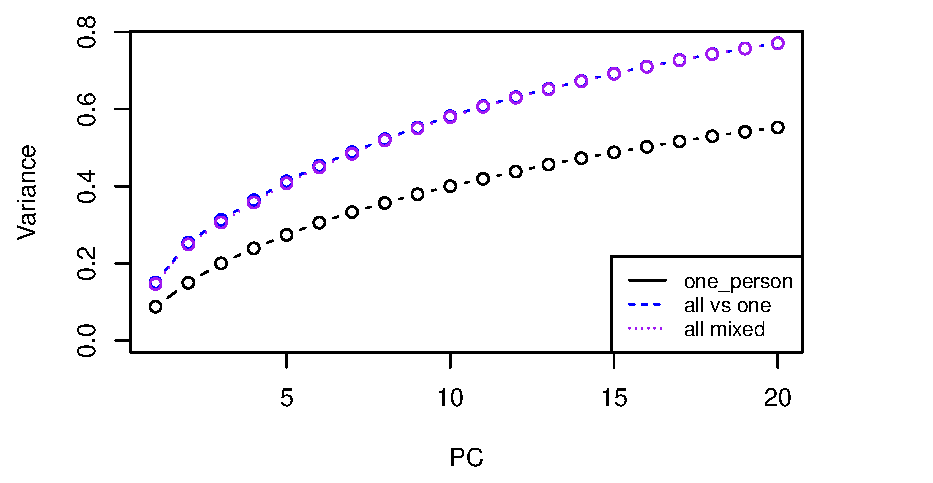
\includegraphics[width=\textwidth]{graphics/pca_acc_variance}
\caption{Accumulated variance.}
\label{fig:pca_accumulated_var}
\end{subfigure}\\[-1cm]
\begin{subfigure}{0.70\textwidth}
\centering
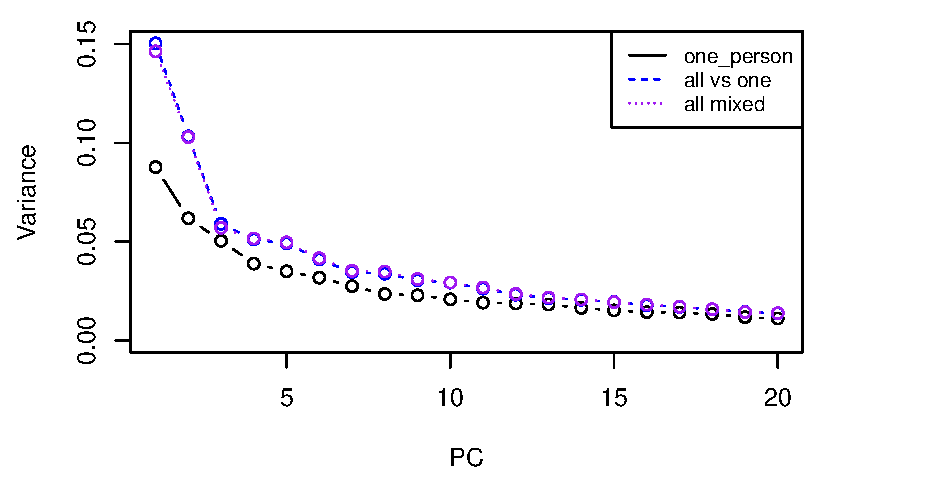
\includegraphics[width=\textwidth]{graphics/pca_variance}
\caption{Variance of a single component.}
\label{fig:pca_var}
\end{subfigure}
\caption[PCA variance.]{Variance for the first 20 principle components.
The data was run on Group 3 member 2's data on 100 DPI. }
\label{fig:variance}
\end{figure}
% Figure \ref{fig:contour_KvsPCA_G3M2vsRest} shows a contour plot of how well Group 3 Member 2's  handwriting was predicted successfully for $K$ and the total variance represented of the PC's varying between one and 20 and 0.5 and 1 respectively.


The variance can also be plotted using the same data, but normalized using z-score first.
This is illustrated on figure \ref{fig:variance_zscore}.




\begin{figure}[H]
\centering
\begin{subfigure}{0.70\textwidth}
\centering
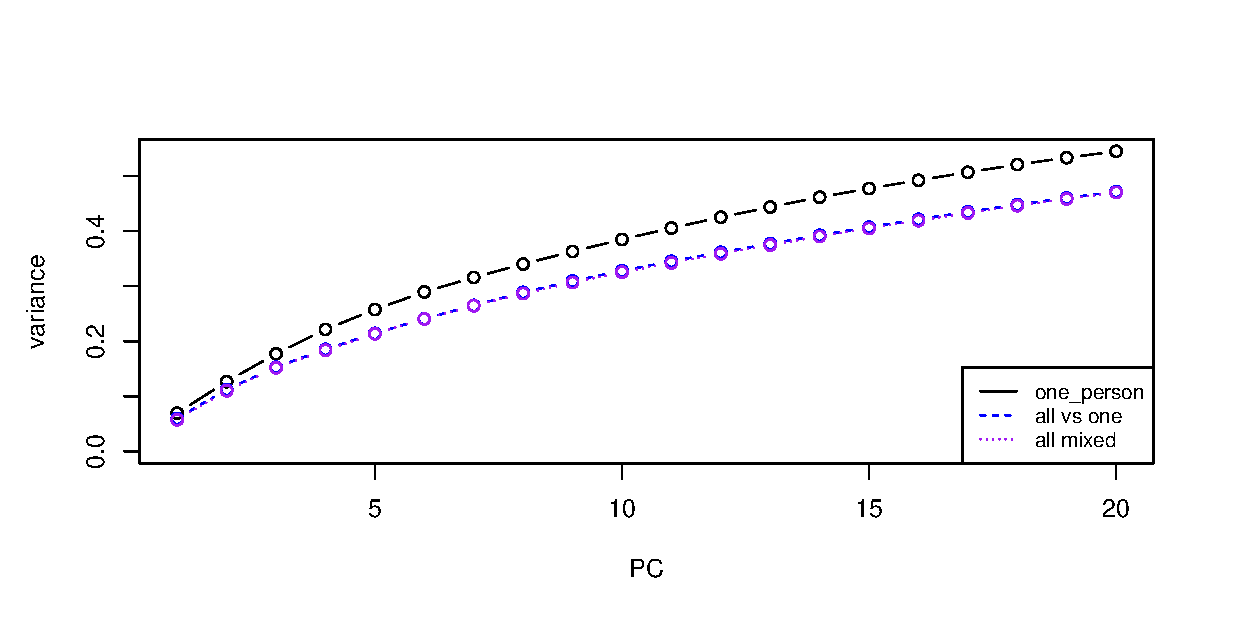
\includegraphics[width=\textwidth]{graphics/pca_acc_variance_zs}
\caption{Accumulated variance.}
\label{fig:pca_accumulated_var_zscore}
\end{subfigure}\\[-1cm]
\begin{subfigure}{0.70\textwidth}
\centering
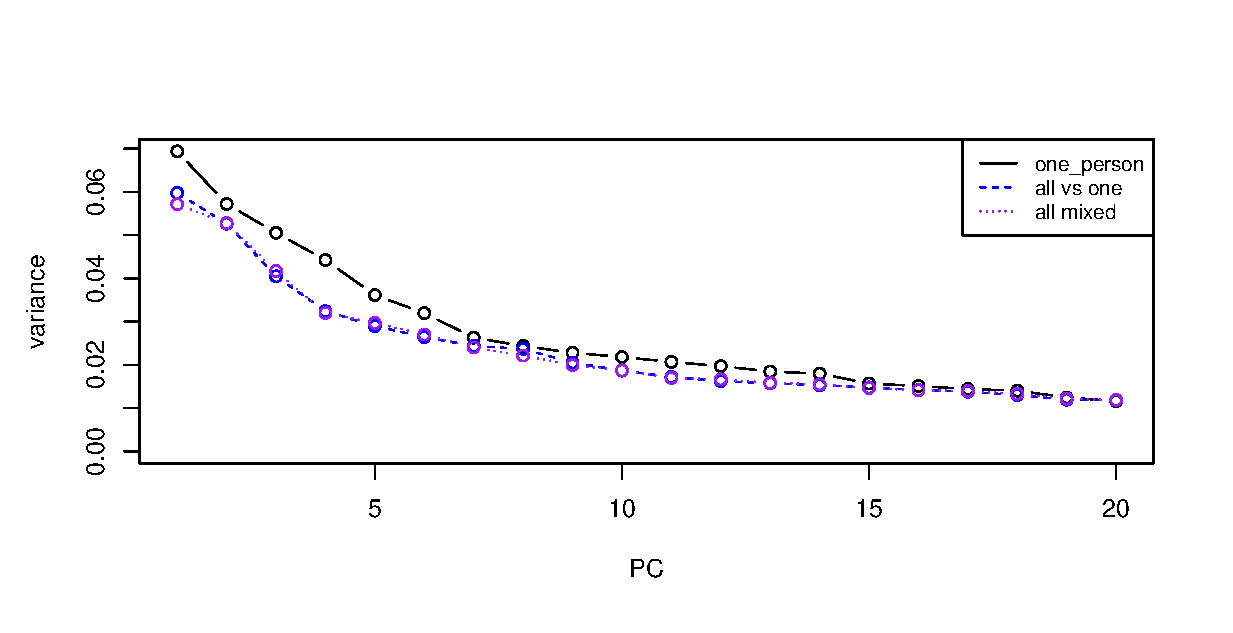
\includegraphics[width=\textwidth]{graphics/pca_variance_zs}
\caption{Variance of a single component.}
\label{fig:pca_var_zscore}
\end{subfigure}
\caption[PCA variance when data is normalized using z-score.]{Variance for the first 20 principle components on a z-score normalized dataset.
The data was run on Group 3 member 2's data on 100 DPI. }
\label{fig:variance_zscore}
\end{figure}


The effect of using z-score can be seen on the two graphs.
It is clear that the variance of the first PC in figure \ref{fig:pca_var} is considerably higher than that of figure \ref{fig:pca_var_zscore} for all three tests.
As the number of components increases, the two curves for the one-person test catches up to the higher in figure \ref{fig:pca_accumulated_var_zscore} which was not normalized.
However, the results for the two other test sets show that the accumulative variance in the case of using z-score averages the variance amongst the components more.
This results in the first few components being less significant than when not using z-score, but the lower PC have a higher level of significance.
Furthermore a larger set of PC are necessary to represent the same variance when using PCA with z-score applied beforehand than when not using it.






\newpage
\section{K-NN}
\section{Introduction}

The classification of handwritten characters is used in a wide range of products to day.
Hence, this report goes in depth with how the numbers from zero to nine can be classified using machine learning algorithms.

The data set consists of a set of handwritten characters from zero to nine.
These were constructed by the students enrolled in the course Statistical Machine learning (RM-SML-E1) in 2015 at the University of Southern Denmark (SDU).
The characters were written in boxes of $0.55 \times 0.55 \textit{ cm}$ on a sheet with $20 \times 20$ boxes for each character.
The set used in this report is the 100DPI dataset.
Each number is hence stored as a $20 \times 20 \textit{ pixel}$ matrix containing the handwritten character.

The methods used for classification are K-Nearest Neighbours and Decision Trees.
This is to compare a method of lazy supervised learning against a method of supervised learning.
Furthermore a set of different ways to pre-process the data is explored.
Finally the two methods are compared with each at the best parameters and preprocessing settings.

The goal is to tests the handwritten digits from 20 people enrolled in the course.
The first test is where all people are mixed together, everybody contributing 90\% of their data to the training set and 10\% to the test set.
This is considered the easy problem as special ways of writing a digit will be represented in the training data.

Another test is to use 19 people's digits as training data and use the last person to test.
This is considered the hard problem.

To test the performance of the classification methods a simplified problem has been constructed.
It takes training data from a single person, Lukas Schwartz, which is referred to as Group 3 member 2 (G3M2).
By splitting the data 90\% for training and 10\% for testing
360 digits from each class as training data and 40 digits was used.
Testing each parameter with the simplified problem means the parameters could be tested in less time than if using the entire data set.


\subsection{K-NN Theory}
The K-Nearest Neighbour (K-NN) method is in this report used to classify a specific unknown character to a set of characters ranging from 0 to 9.
The method utilizes the euclidean distance to the nearest characters


\subsection{Parameter Tuning}



\begin{figure}[H]
\centering
\missingfigure{number of tunings vs smoothing}
\end{figure}


\begin{figure}[H]
\centering
\missingfigure{number of tunings vs pca (+/- z.s.)}
\end{figure}


\begin{figure}[H]
\centering
\missingfigure{number of tunings vs entropy or z.s.}
\end{figure}


\begin{figure}[H]
\centering
\missingfigure{timing of tunings vs pca and no trees}
\end{figure}


\begin{figure}[H]
\centering
\missingfigure{number of trees vs smoothing}
\end{figure}


\begin{figure}[H]
\centering
\missingfigure{number of trees vs pca (+/- z.s.)}
\end{figure}


\begin{figure}[H]
\centering
\missingfigure{number of trees vs entropy or z.s.}
\end{figure}


\begin{figure}[H]
\centering
\missingfigure{timing of no trees vs pca }
\end{figure}

\subsection{Conclusion}



Multiple test were performed to find the best possible way to optimize the time taken to run and the success gained from using the K-NN algorithm.
It was chosen to use 40 PC to optimize speed, while keeping a descend success rate.
Furthermore it was found to benefit the success rate when smoothing the data using a Gaussian filter with sigma of 0.9 and a filter size of 5.
The success rate was also improved by applying z-score normalization.



\newpage
\section{Decision Trees}
\section{Introduction}

The classification of handwritten characters is used in a wide range of products to day.
Hence, this report goes in depth with how the numbers from zero to nine can be classified using machine learning algorithms.

The data set consists of a set of handwritten characters from zero to nine.
These were constructed by the students enrolled in the course Statistical Machine learning (RM-SML-E1) in 2015 at the University of Southern Denmark (SDU).
The characters were written in boxes of $0.55 \times 0.55 \textit{ cm}$ on a sheet with $20 \times 20$ boxes for each character.
The set used in this report is the 100DPI dataset.
Each number is hence stored as a $20 \times 20 \textit{ pixel}$ matrix containing the handwritten character.

The methods used for classification are K-Nearest Neighbours and Decision Trees.
This is to compare a method of lazy supervised learning against a method of supervised learning.
Furthermore a set of different ways to pre-process the data is explored.
Finally the two methods are compared with each at the best parameters and preprocessing settings.

The goal is to tests the handwritten digits from 20 people enrolled in the course.
The first test is where all people are mixed together, everybody contributing 90\% of their data to the training set and 10\% to the test set.
This is considered the easy problem as special ways of writing a digit will be represented in the training data.

Another test is to use 19 people's digits as training data and use the last person to test.
This is considered the hard problem.

To test the performance of the classification methods a simplified problem has been constructed.
It takes training data from a single person, Lukas Schwartz, which is referred to as Group 3 member 2 (G3M2).
By splitting the data 90\% for training and 10\% for testing
360 digits from each class as training data and 40 digits was used.
Testing each parameter with the simplified problem means the parameters could be tested in less time than if using the entire data set.


\subsection{Entropy}
To compute the optimum decision point for the individual principle components, the entropy method is used.
The entropy of the PC's with our ten ciphers is given by equation \ref{eq:entropy}.

\begin{equation}
Entropy(S) = \sum_{i = '0'}^{'9'} -p_i \cdot \log_2(p_i) 
\qquad \because p_i = P(x = i)
\label{eq:entropy}
\end{equation}

To find the best decision point, it is wanted that the entropy of the two resulting systems, when dividing one PC into two, is as low as possible.
This can be represented as sum of entropy for our two resulting datasets, weighted by the relative size of such.
This is given in equation \ref{eq:entropy_datasetdevision}.

\begin{eqnarray}
Entropy = \sum_{i = 1}^{2} \frac{s_i \cdot Entropy(S_i)}{\sum_{k = 1}^{2} s_k} 
\qquad \because S_i \subset S\ and\ s_k = size(S_k)
\label{eq:entropy_datasetdevision}
\end{eqnarray}

When using equation \ref{eq:entropy_datasetdevision} on the first five principle components on the data of 15 people from the class, then figure \ref{fig:entropy_pc5} was gained.

\begin{figure}[H]
\centering
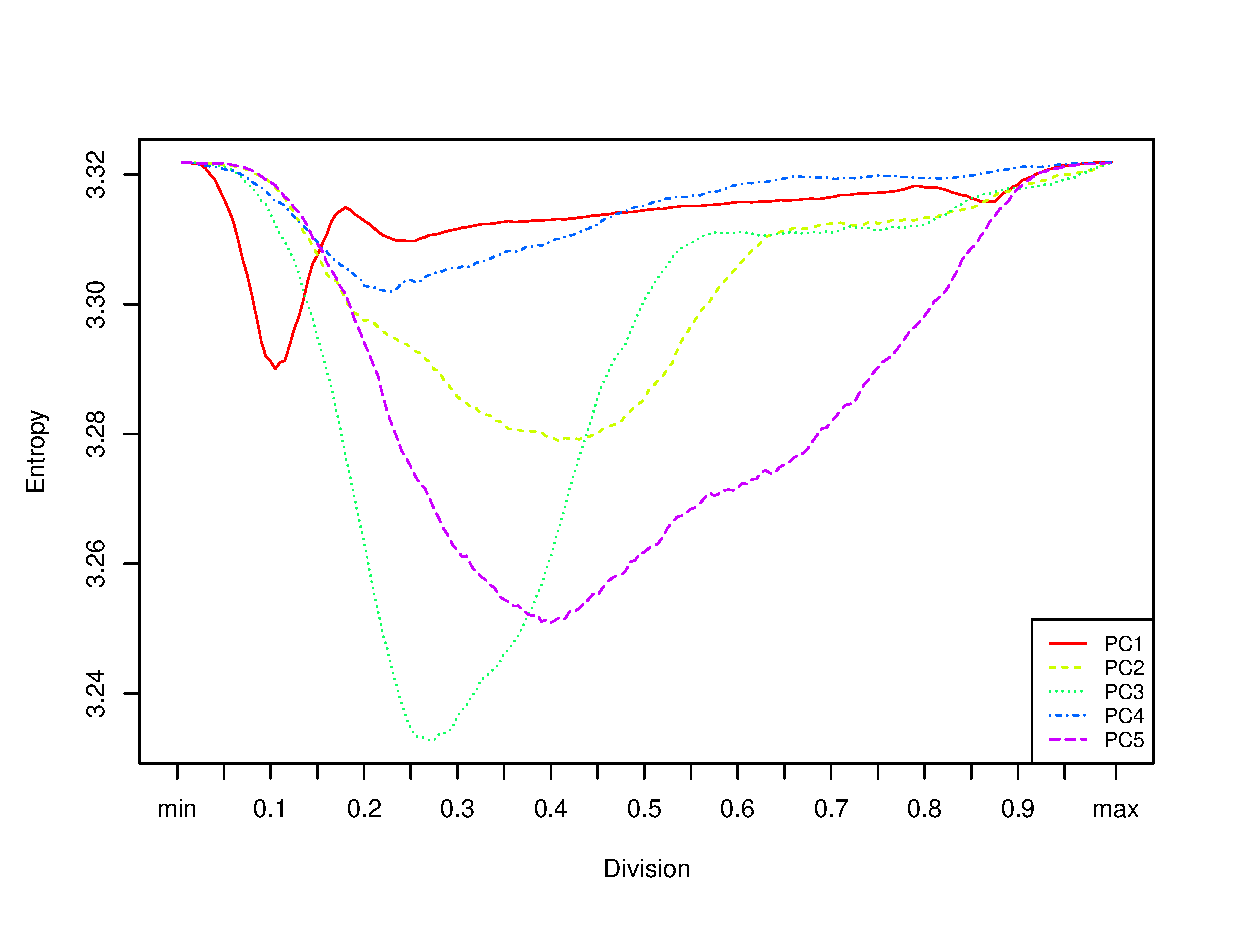
\includegraphics[width = 0.9 \textwidth]{graphics/entropy_pc}
\caption[Variation of the entropy]{Figure showing the variation of the entropy of the dataset when the decision point varies. Computed using equation \ref{eq:entropy_datasetdevision}. The data of the first five principle component.}
\label{fig:entropy_pc5}
\end{figure}


The point of lowest entropy for a principle component was then used as the splitting point to convert the data into binary.
This was done by setting everything below the splitting point to true and the rest false.
This was then done for all principle components on both the test and train set. 
The splitting point for the components in the test set were taken as the splitting point from the same component in the train set.

The optimal decision decision point is shown along with the PC values for PC1 in figure \ref{fig:decision_point}. 
The different data rows represent the ten different characters (from zero to nine).
Here it is clear that if the data is above the split then it is highly unlikely to be a 0.
If the data is below, further investigation is needed.
By removing all unlikely classes the true class must remain.

\begin{figure}[H]
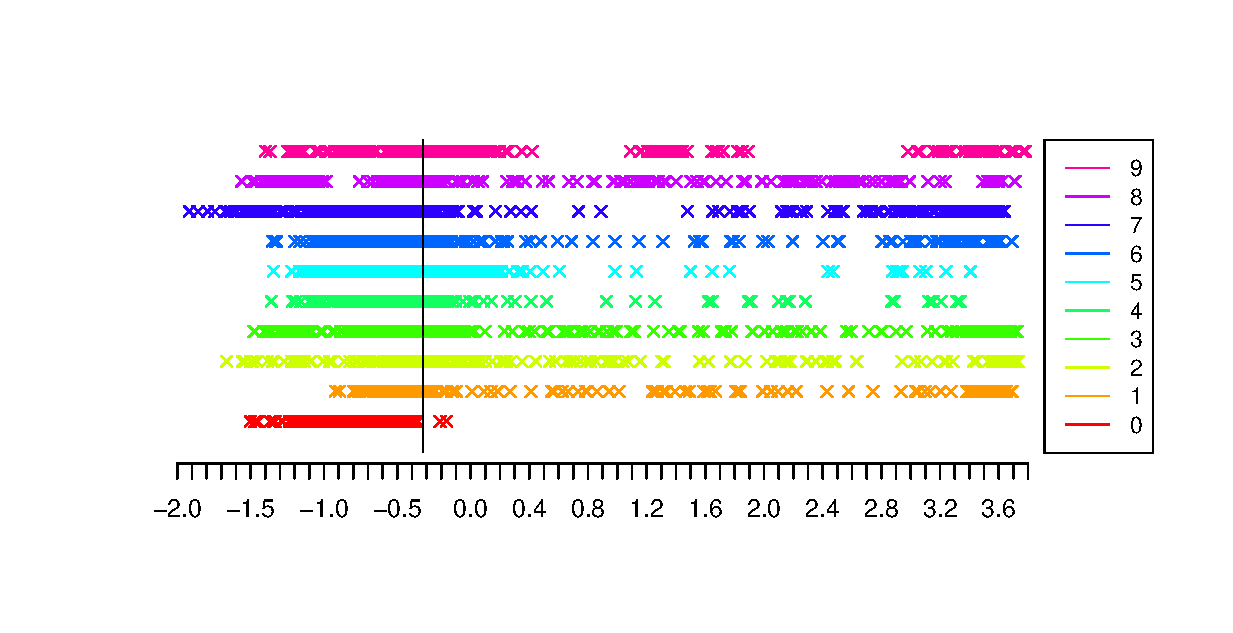
\includegraphics[width = \textwidth]{graphics/decision_seperation}
\caption{Decision point in relation to PC values.}
\label{fig:decision_point}
\end{figure}






\subsection{K-NN Theory}
The K-Nearest Neighbour (K-NN) method is in this report used to classify a specific unknown character to a set of characters ranging from 0 to 9.
The method utilizes the euclidean distance to the nearest characters


\subsection{Parameter Tuning}



\begin{figure}[H]
\centering
\missingfigure{number of tunings vs smoothing}
\end{figure}


\begin{figure}[H]
\centering
\missingfigure{number of tunings vs pca (+/- z.s.)}
\end{figure}


\begin{figure}[H]
\centering
\missingfigure{number of tunings vs entropy or z.s.}
\end{figure}


\begin{figure}[H]
\centering
\missingfigure{timing of tunings vs pca and no trees}
\end{figure}


\begin{figure}[H]
\centering
\missingfigure{number of trees vs smoothing}
\end{figure}


\begin{figure}[H]
\centering
\missingfigure{number of trees vs pca (+/- z.s.)}
\end{figure}


\begin{figure}[H]
\centering
\missingfigure{number of trees vs entropy or z.s.}
\end{figure}


\begin{figure}[H]
\centering
\missingfigure{timing of no trees vs pca }
\end{figure}

\subsection{Conclusion}



Multiple test were performed to find the best possible way to optimize the time taken to run and the success gained from using the K-NN algorithm.
It was chosen to use 40 PC to optimize speed, while keeping a descend success rate.
Furthermore it was found to benefit the success rate when smoothing the data using a Gaussian filter with sigma of 0.9 and a filter size of 5.
The success rate was also improved by applying z-score normalization.



\newpage
\section{Algorithm Comparison}
\section{Introduction}

The classification of handwritten characters is used in a wide range of products to day.
Hence, this report goes in depth with how the numbers from zero to nine can be classified using machine learning algorithms.

The data set consists of a set of handwritten characters from zero to nine.
These were constructed by the students enrolled in the course Statistical Machine learning (RM-SML-E1) in 2015 at the University of Southern Denmark (SDU).
The characters were written in boxes of $0.55 \times 0.55 \textit{ cm}$ on a sheet with $20 \times 20$ boxes for each character.
The set used in this report is the 100DPI dataset.
Each number is hence stored as a $20 \times 20 \textit{ pixel}$ matrix containing the handwritten character.

The methods used for classification are K-Nearest Neighbours and Decision Trees.
This is to compare a method of lazy supervised learning against a method of supervised learning.
Furthermore a set of different ways to pre-process the data is explored.
Finally the two methods are compared with each at the best parameters and preprocessing settings.

The goal is to tests the handwritten digits from 20 people enrolled in the course.
The first test is where all people are mixed together, everybody contributing 90\% of their data to the training set and 10\% to the test set.
This is considered the easy problem as special ways of writing a digit will be represented in the training data.

Another test is to use 19 people's digits as training data and use the last person to test.
This is considered the hard problem.

To test the performance of the classification methods a simplified problem has been constructed.
It takes training data from a single person, Lukas Schwartz, which is referred to as Group 3 member 2 (G3M2).
By splitting the data 90\% for training and 10\% for testing
360 digits from each class as training data and 40 digits was used.
Testing each parameter with the simplified problem means the parameters could be tested in less time than if using the entire data set.



\section{Conclusion}

\subsection{Worst Handwriting}


\newpage


% \section{K-Nearest Neighbours}
% 
% % % % Part one
% \subsection{K-NN Theory}
The K-Nearest Neighbour (K-NN) method is in this report used to classify a specific unknown character to a set of characters ranging from 0 to 9.
The method utilizes the euclidean distance to the nearest characters


% 
% % \subsection{K-NN Implementation}
The K-NN algorithm is implemented as in code \ref{code:KNN_implementation}.
The implementation of how the result of the voting is calculated, is not shown here.


\lstinputlisting[language = R,
firstnumber = 291,
firstline = 291, 
lastline = 311, 
captionpos=b,
caption = {K-NN implementation.},
label = {code:KNN_implementation}]{../Code/KNN/01/test.R}


The function takes three arguments, \texttt{testVector}, \texttt{trainVectors} and \texttt{k}. 
\texttt{testVector} is a vector containing the set of pixel values of the character that is wished identified. 
\texttt{trainVectors} is a three dimensional set of vectors. 
This makes it possible to distinguish between the character represented by the group and the individual characters and their data.

Line 290 to 293, in code \ref{code:KNN_implementation}, defines the two arrays \texttt{neighbours} and \texttt{testDistance}.
These are used to store the \texttt{k} nearest neighbours and calculate the distance between two characters respectively.

The code then, in line 295 to 299, loops through all the different character groups and the characters within.
For each character the distance is then calculated to the \texttt{testVector}.
If the distance is smaller than that of one of the previously inserted into \texttt{neighbours}, 
then lines 301 to 309 insert it into the \texttt{neighbours} list in sorted order and the one furthest away is removed.

Once this is done, the \texttt{neighbours} list can then be inspected to guess which character it is.
% 
% \subsection{Person Dependent}
This section tests the KNN algorithm explained earlier using data from one single person, namely Group three member two's data.
The test are performed first with the data split equally into a 50\% for the training and 50\% for the test set.
Afterwards with a 90/10\% split for training and test respectively is computed.
Both test where conducted using cross validation with 10 runs.

\subsubsection{Equally Sized training and test set}
Figure \ref{fig:PersonDependentPerformance_5050} shows a test with 50/50\% split was carried out for changing \textit{K}'s.

\begin{figure}[H]
\centering
% figure...
\caption{Test result with a 50/50\% split of group three member two's data with changing values for \textit{K}. The data points are taken as the mean of 10 runs using cross validation.}
\label{fig:PersonDependentPerformance_5050}
\end{figure}

As seen on figure \ref{fig:PersonDependentPerformance_5050} then \textbf{...}.


\subsubsection{90/10 Data Split}
A cross validation was also carried out using a 90/10\% split of the data. 
The result of this is seen in figure \ref{fig:PersonDependentPerformance_9010}.


\begin{figure}[H]
\centering
% figure...
\caption{Test result with a 90/10\% split of group three member two's data with changing values for \textit{K}. The data points are taken as the mean of 10 runs using cross validation.}
\label{fig:PersonDependentPerformance_9010}
\end{figure}

Figure \ref{fig:PersonDependentPerformance_9010} \textbf{...}.


% 
% % 1.6.2: tabel over mean+var over 10 runs + 
%        graf dpi vs success for filtre (10 run)

\subsection{Preprocessed Image - Single Person Tests}

\begin{table}[h]
\centering
    \begin{subtable}[b]{0.56\textwidth}
    \centering
        \begin{tabular}{lcccccc}
            &Raw	& Avg	& G 0.5	& G 1	& G 2 \\
\hline
100	& 0.8297	& 0.8297	& 0.8788	& 0.8545	& 0.7750 \\
200	& 0.8635	& 0.8635	& 0.9180	& 0.8998	& 0.8602 \\
300	& 0.8925	& 0.8925	& 0.9373	& 0.9190	& 0.8842 \\

        \end{tabular}
        \caption{Mean success rate.}
    \end{subtable}
    \begin{subtable}[b]{0.56\textwidth}
    \centering
        \begin{tabular}{lcccccc}
            &Raw	& Avg	& G 0.5	& G 1	& G 2 \\
\hline
100	& 0.83	& 0.83	& 0.86	& 0.85	& 0.78 \\
200	& 0.86	& 0.86	& 0.90	& 0.90	& 0.86 \\
300	& 0.89	& 0.89	& 0.92	& 0.92	& 0.88 \\

        \end{tabular}
        \caption{Variance in success rate.}
    \end{subtable}
    \caption[Success of smoothing functions.]{Mean success rate and variance of different smoothing functions.}
    \label{tb:smooth}
\end{table}

\begin{figure}[h]
\centering
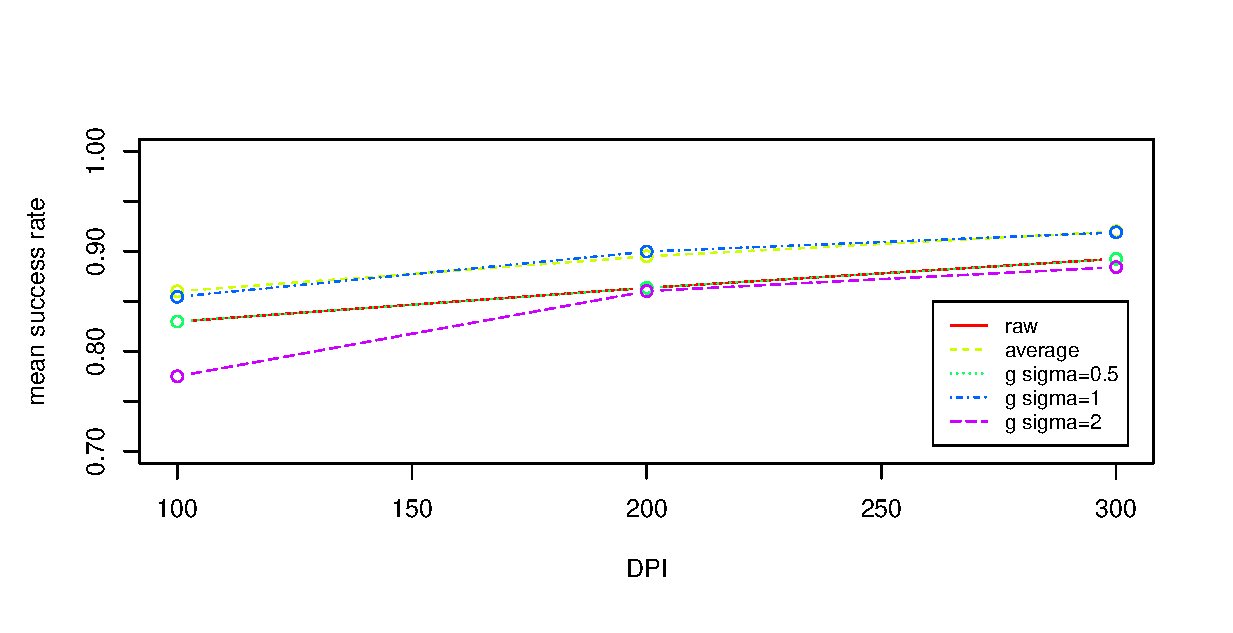
\includegraphics[width=1\textwidth]{graphics/smoothing}
\caption{Success rate of smoothing functions.}
\label{fig:smooth}
\end{figure}

Applying a smoothing function can give the image an advantage when using the nearest neighbour analysis.
By taking an average of the neighbouring pixels the lines in the digit should be wider and the digits should have a better chance of overlapping.
The danger is that too much smoothing could make the whole image one colour and would completely destroy any chance of analysis.
A Gaussian distribution (also referred to as a normal distribution) a naturally occurring distribution that happens when a random result occurs around a mean. 
The $\sigma$ signifies the deviation of the distribution. 
The 2D equation of a Gaussian distribution is shown in equation \ref{eq:gauss}. 

\begin{equation}
G(x,y) = \frac{1}{2\pi \sigma^2} e^{- \frac{x^2+y^2}{2\sigma^2}} \label{eq:gauss}
\end{equation}

Using the Gaussian filter to smooth an image will weigh the distance to the pixel.
A small $\sigma$ will make a small deviation and thus heavily weigh the center pixel.
The results of the filtering methods were also compared to the raw image with 100, 200 and 300 DPI.
These results are compared with an averaging filter (avg) which takes the average of the four neighbouring pixels and a Gaussian filter (G) with different values for sigma.
These tests were done 10 times, using cross validation, and the mean of each success rate is plotted in figure \ref{fig:smooth}. 
Since the variance is too small to be seen in the figure the mean and variance is shown in table \ref{tb:smooth}.
The averaging filter does not give a measurable different result from not using a filter.
The Gaussian filter does improves the success rate for some values of sigma, but a larger $\sigma$ makes it worse.

% 
% %\section{K-NN on Big Data}
% \section{Introduction}

The classification of handwritten characters is used in a wide range of products to day.
Hence, this report goes in depth with how the numbers from zero to nine can be classified using machine learning algorithms.

The data set consists of a set of handwritten characters from zero to nine.
These were constructed by the students enrolled in the course Statistical Machine learning (RM-SML-E1) in 2015 at the University of Southern Denmark (SDU).
The characters were written in boxes of $0.55 \times 0.55 \textit{ cm}$ on a sheet with $20 \times 20$ boxes for each character.
The set used in this report is the 100DPI dataset.
Each number is hence stored as a $20 \times 20 \textit{ pixel}$ matrix containing the handwritten character.

The methods used for classification are K-Nearest Neighbours and Decision Trees.
This is to compare a method of lazy supervised learning against a method of supervised learning.
Furthermore a set of different ways to pre-process the data is explored.
Finally the two methods are compared with each at the best parameters and preprocessing settings.

The goal is to tests the handwritten digits from 20 people enrolled in the course.
The first test is where all people are mixed together, everybody contributing 90\% of their data to the training set and 10\% to the test set.
This is considered the easy problem as special ways of writing a digit will be represented in the training data.

Another test is to use 19 people's digits as training data and use the last person to test.
This is considered the hard problem.

To test the performance of the classification methods a simplified problem has been constructed.
It takes training data from a single person, Lukas Schwartz, which is referred to as Group 3 member 2 (G3M2).
By splitting the data 90\% for training and 10\% for testing
360 digits from each class as training data and 40 digits was used.
Testing each parameter with the simplified problem means the parameters could be tested in less time than if using the entire data set.

% %% % Part two
% \subsection{K-NN on Big Data}
The K-NN algorithm can be seen to be approximately linear on figure \ref{fig:predictionTimeVStrainSize}.
It takes approximately 0.47 seconds to predict a single value.

\begin{figure}[H]
\centering
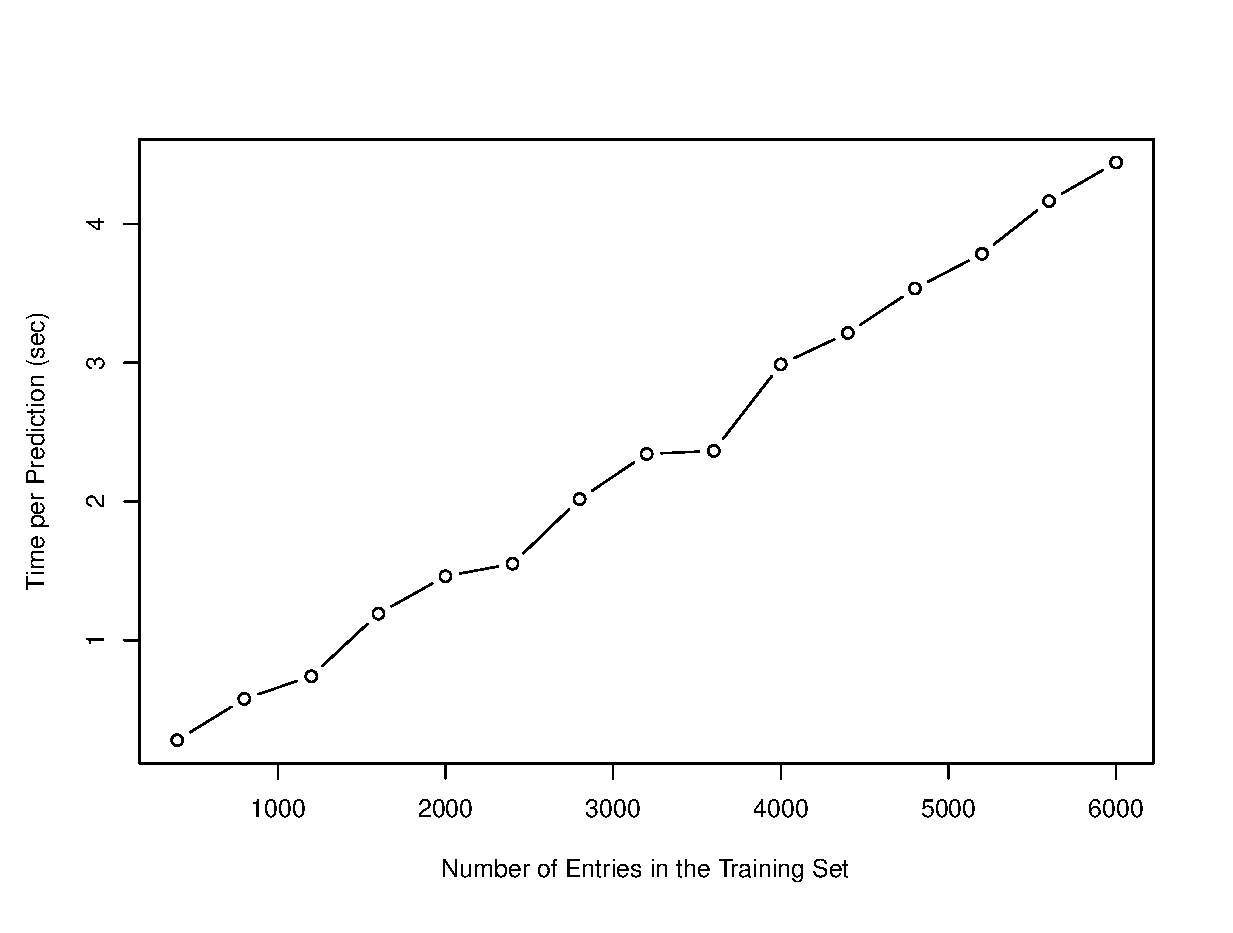
\includegraphics[width = 0.95 \textwidth]{graphics/graph_timeVSppl}
\caption{The time taken for one prediction for different training set sizes at 100 DPI resolution.}
\label{fig:predictionTimeVStrainSize}
\end{figure}

This can, when a lot of values, such as the 4000 elements dataset of a single person, take a long time to predict all of them (approx. 30 min on 100 DPI).
It is therefore desirable to bring down the prediction time.
This will be considered in the following chapters.

% %
% \subsection{Principle Component Analysis}


\begin{figure}[H]
\centering
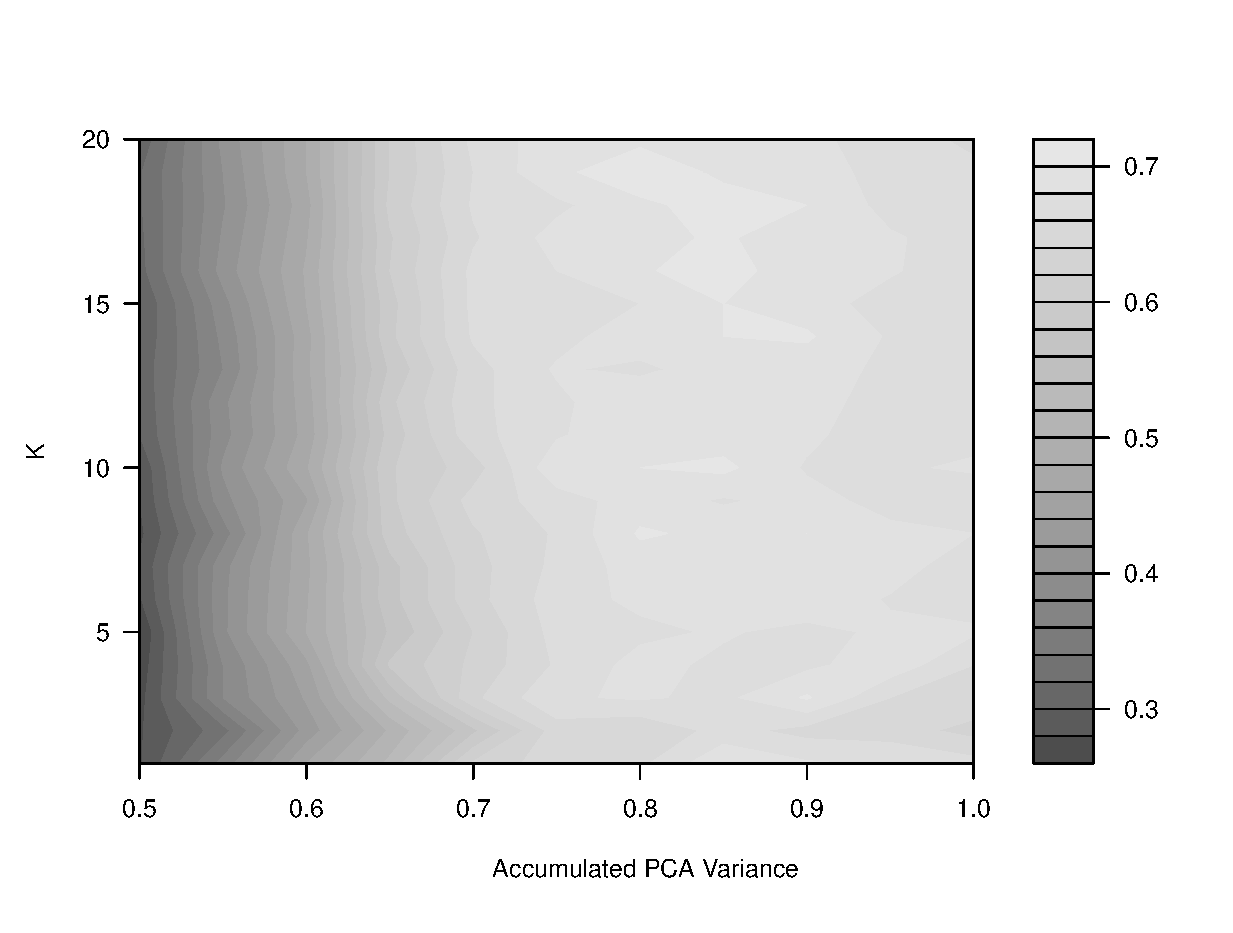
\includegraphics[width = 16cm]{graphics/contour_k_PCA_oneVsRest}
\caption{Success rate for detection of characters of Group 3 Member 2's data when he himself is not represented in the training set. 
Thewas tested with 16 people.}
\label{fig:}
\end{figure}


\begin{figure}
\centering
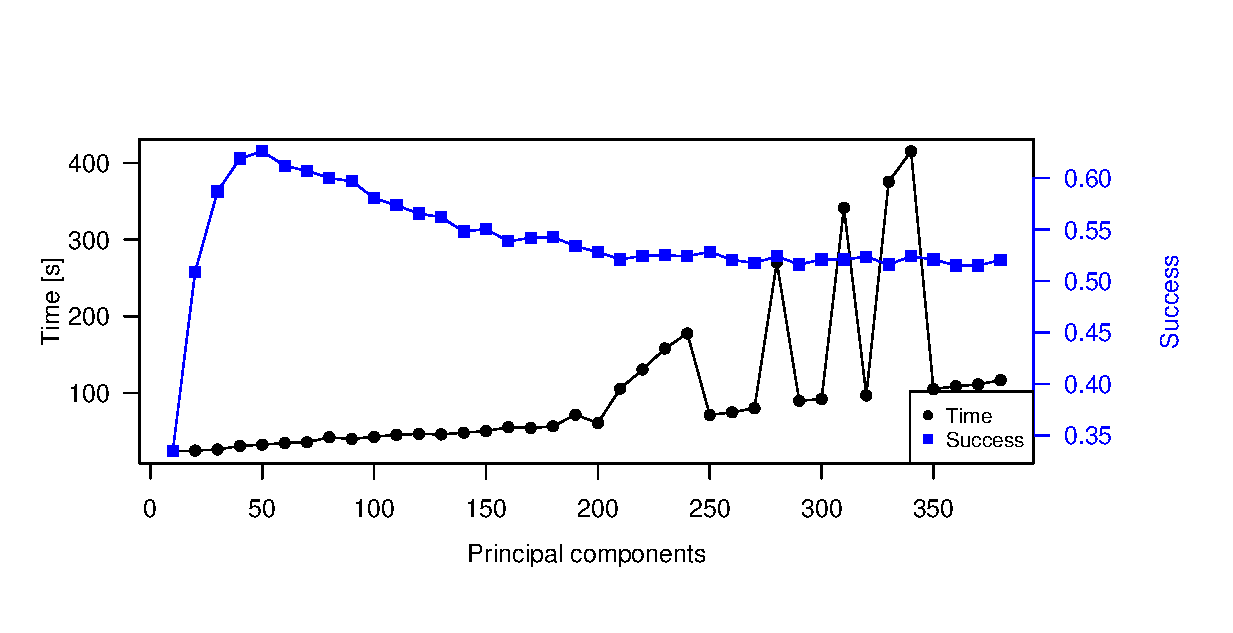
\includegraphics[width =0.8 \textwidth]{graphics/pca_timing}
\caption{Timing of running the PCA with different principle components. 
The data was run on Group 3 member 1's data on 100 DPI. 
The percentage of successful predictions is also measured with the same data.}
\label{fig:pca_timing}
\end{figure}

\begin{figure}
\centering
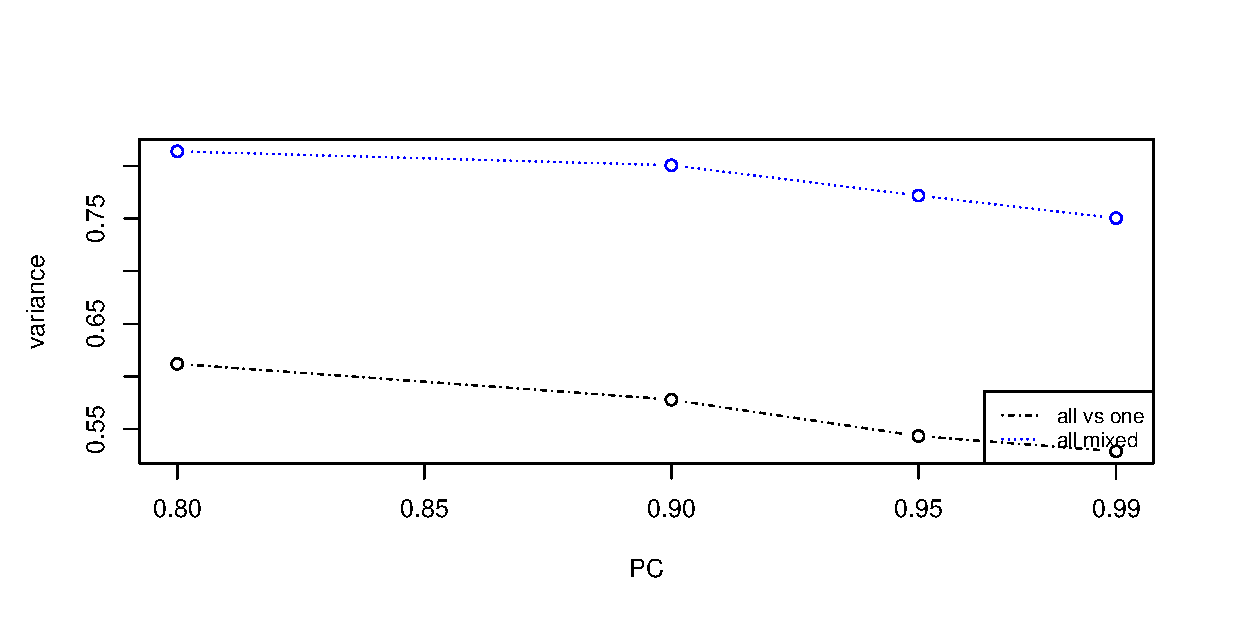
\includegraphics[width =0.8 \textwidth]{graphics/pca_success}
\caption{Percentage of successful predictions with increasing percentage of principle components used.
The data was run on Group 3 member 1's data on 100 DPI. }
\label{fig:pca_success}
\end{figure}


% %
% \subsection{Data Normalization}
\label{sec:DataNormalization}
When comparing multiple entries in a dataset, it might be beneficial to normalize such to obtain a basis for equal comparison.
In the case of numbers being written and detected, such as ours, there might be differences in the colors of the characters when different pens/pencils are used.
This can create unwanted differences between elements in a category, which are else identically, and hence lead to false predictions.
Two normalization algorithms where hence implemented.
These are, min-max normalization and z-score standardization.

Figure \ref{fig:normalization_test_pre-post} shows the result when cross validation is carried out on the data from the 16 people in the class.
In figure \ref{fig:normalization_test_pre-post}, each individual is tested up against the rest of the group without contributing to the training set themselves. 
The two types of normalization are performed both before and after the data reduction using PCA.


\begin{figure}[H]
\centering
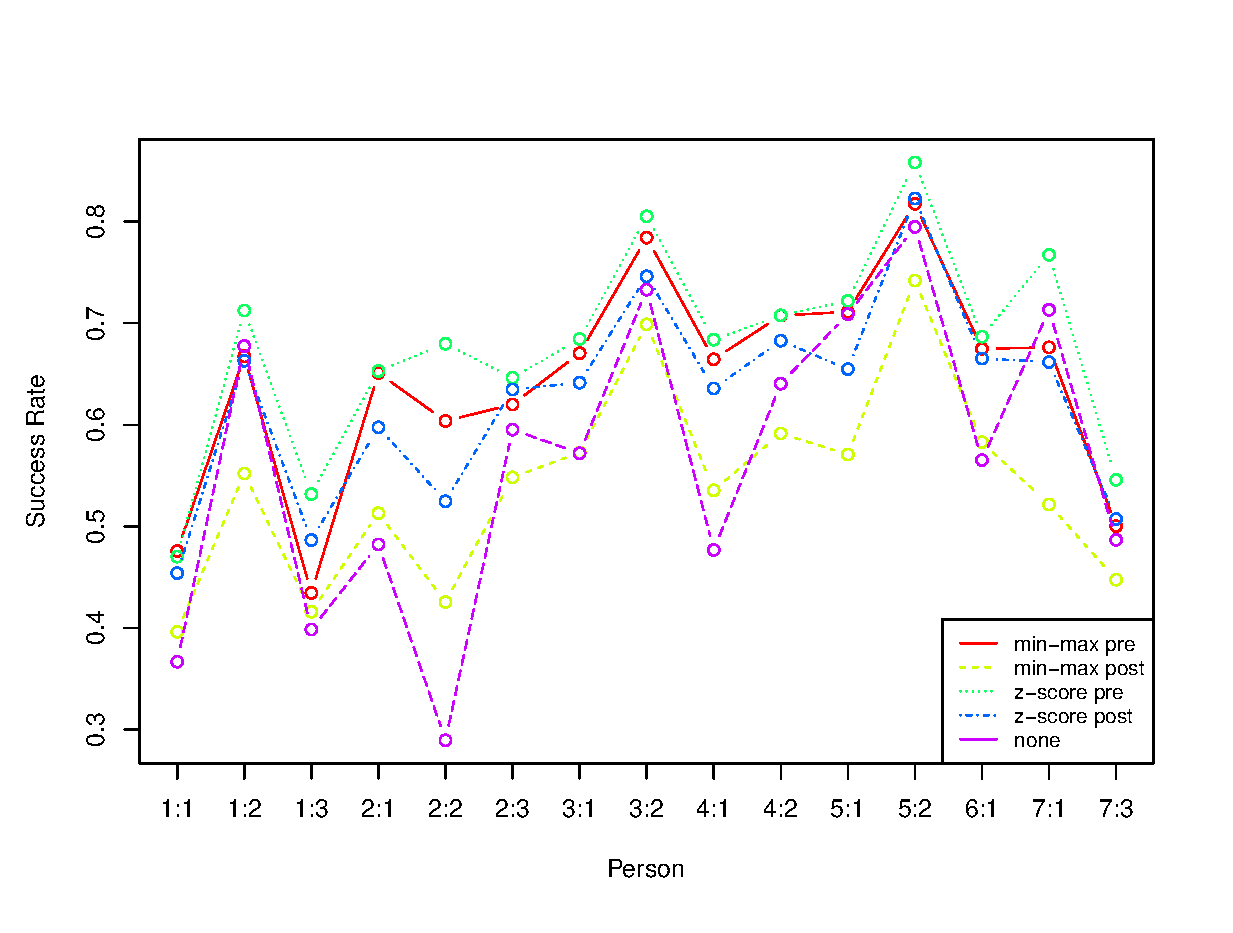
\includegraphics[width = \textwidth]{graphics/graph_normalization}
\caption[Comparison of different students.]{Success rate for detection of characters of on person when not in the training set. 
Data normalized before (pre) and after (post) dataset reduction using PCA.
PCA was set to ensure that 80\% of all variance was included in the data set and K as 10.
The person tested for is given as 'Group':'Member'.
It was tested with 16 people.}
\label{fig:normalization_test_pre-post}
\end{figure}

The mean success rate of figure \ref{fig:normalization_test_pre-post} is listed in table \ref{tab:meanSuccess_normalization_test_pre-post}.
From both the graph and table, it can be concluded that the z-score standardization before the PCA reduction performs, on average, at least 3\% better than the other methods.

The figure \ref{fig:normalization_test_pre-post} also shows that in general all three normalizations, except for the min-max normalization after PCA reduction, is on average, yielding a higher number of correct predictions.

The normalization before the PCA reductions yields a better result in all cases. 
This may be because it enables the PCA to find the features being more responsible for the decision of which category a element belongs to. 
Some of the performance improvement can be because of features of a low variance in their measured value, have a larger relevance as to what the actual category of the elements are.

\textbf{UPDATE TABLE!}

\begin{table}[H]
\centering
\begin{tabular}{|l|r|}\hline
% 0.5720167 0.4639500 0.6055167 0.5521333 0.5034333
Normalization Method & Mean Success \\ \hline
Min-Max Normalization Pre & 57.2 \% \\ \hline
Min-Max Normalization Post & 46.4 \% \\ \hline
Z-Score Normalization Pre & 60.6 \% \\ \hline
Z-Score Normalization Post & 55.2  \% \\ \hline
No Normalization & 50.3 \% \\ \hline
\end{tabular}
\caption{Mean success rates for normalization test as seen in figure \ref{fig:normalization_test_pre-post}.}
\label{tab:meanSuccess_normalization_test_pre-post}
\end{table}



\subsubsection{Performance Effect when adding a Filter}

\begin{figure}[H]
\centering
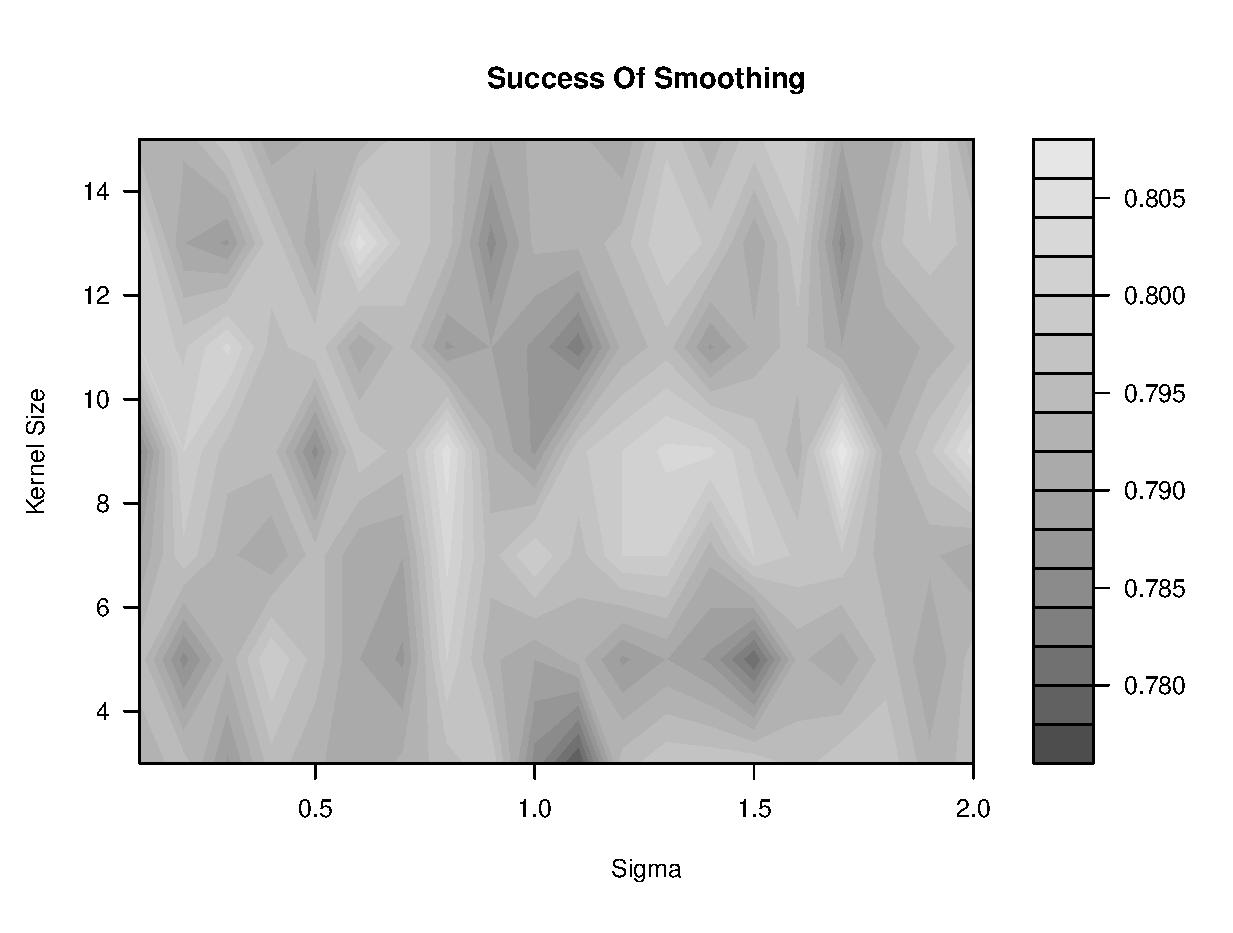
\includegraphics[width = \textwidth]{graphics/success_of_smoothing_contour}
\caption[Optimal smoothing]{Impact of sigma and kernel size when smoothing an image. 
Tested with group 3 member 2's data against 14 other students.
}
\label{fig:smoothing_contour}
\end{figure}

To find the optimal kernel size the success detection rate was plotted with a varying $\sigma$. 
The optimal kernel size is chosen to be 9 pixels wide.
From figure \ref{fig:smoothing_contour} it is concluded that a filter size of 9 is optimal.

Using this knowledge figure \ref{fig:normalization_test_with_smooth} was generated.
The figure compares the unprocessed success rate compared to that of the z-score pre and z-score pre with gaussian smoothing (filter size 9 and sigma 0.7).

 \begin{figure}[H]
 \centering
 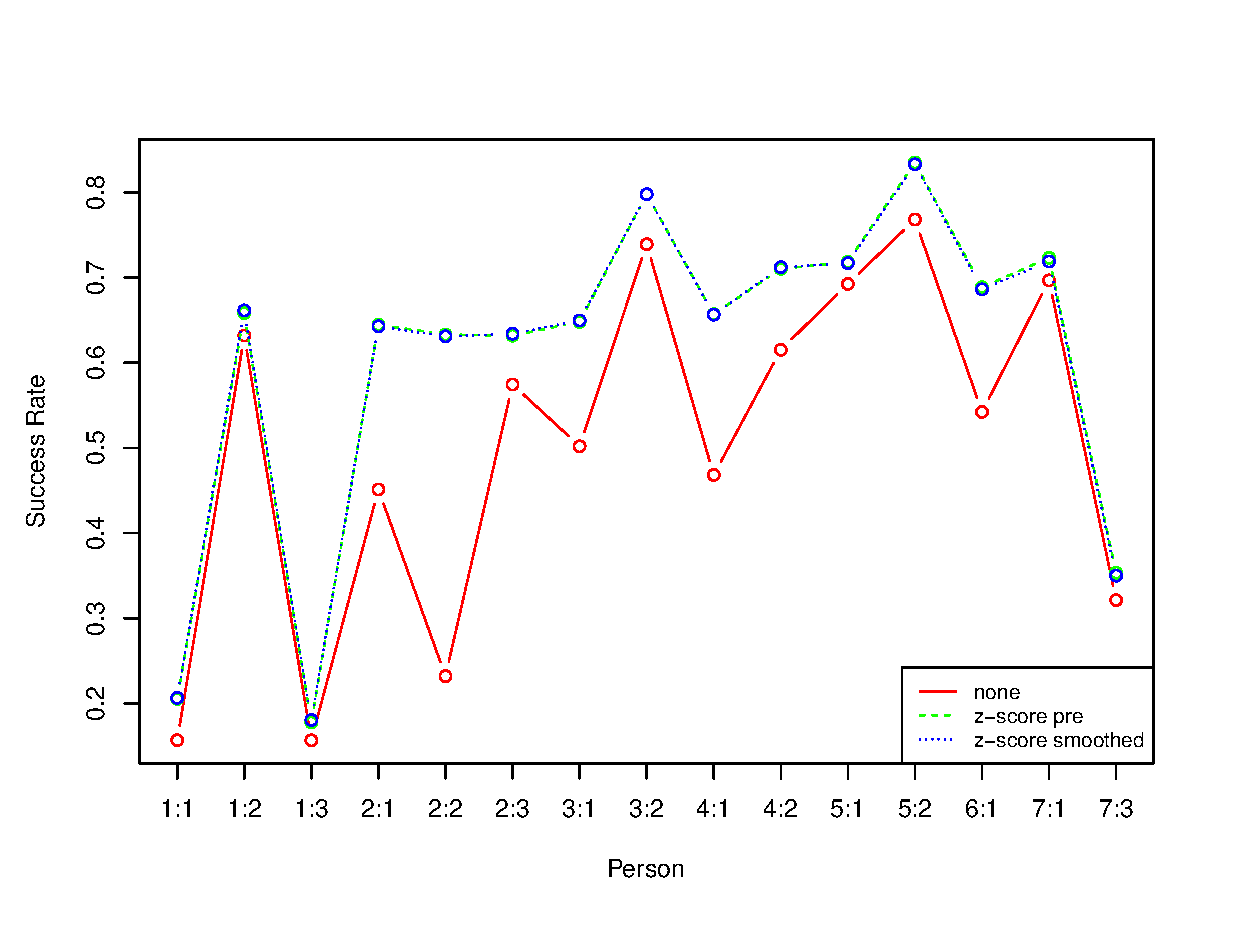
\includegraphics[width = \textwidth]{graphics/graph_normalization_smoothed}
 \caption[Filtered and normalized data.]{Filtered data normalized vs unfiltered normalized data.
 Running each person against the rest of the class in the train set.
 }
 \label{fig:normalization_test_with_smooth}
 \end{figure}

As seen on figure \ref{fig:normalization_test_with_smooth}, then the result of smoothing the data before normalization is not improving the data.

% %
% \subsection{K-means}
K-means is used to group the dataset into categories depending on their location in the x-dimensional space determined by the amount of features representing one of them.
The center of these clusters are then computed and identified as a specific category.
Using these centres, a unknown element can then be categorized depending on which cluster is the closest.

To find the number of clusters best representing the dataset, then the within-group heterogeneity and homogeneity was computed for various K's as seen on figure \textbf{ref!!}.
The elbow point can from here be determined to be at \textbf{K = something}.

\begin{figure}
\centering
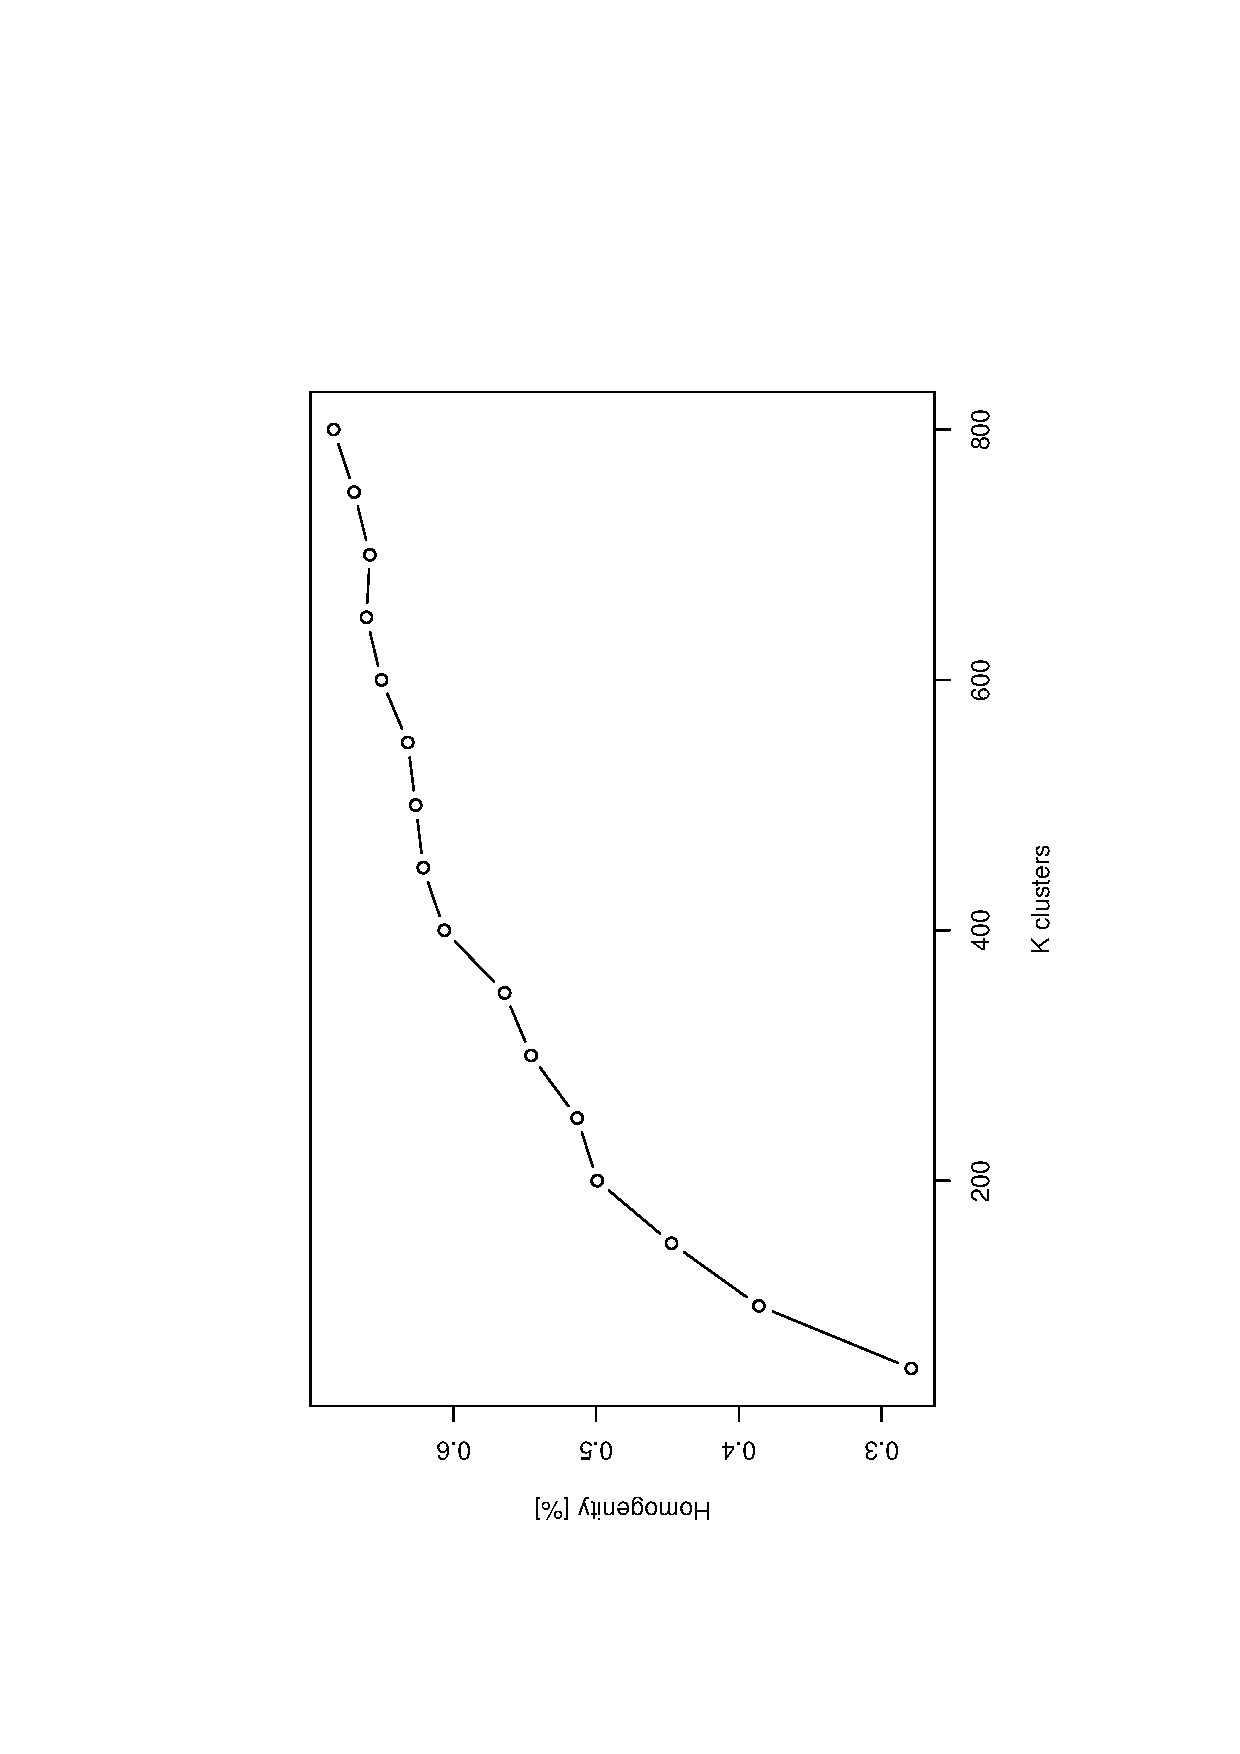
\includegraphics[width=\textwidth]{graphics/homogenity}
\caption{Homogeneity of the data set.}
\label{fig:homogeneity_kmean}
\end{figure}


\begin{figure}
\centering
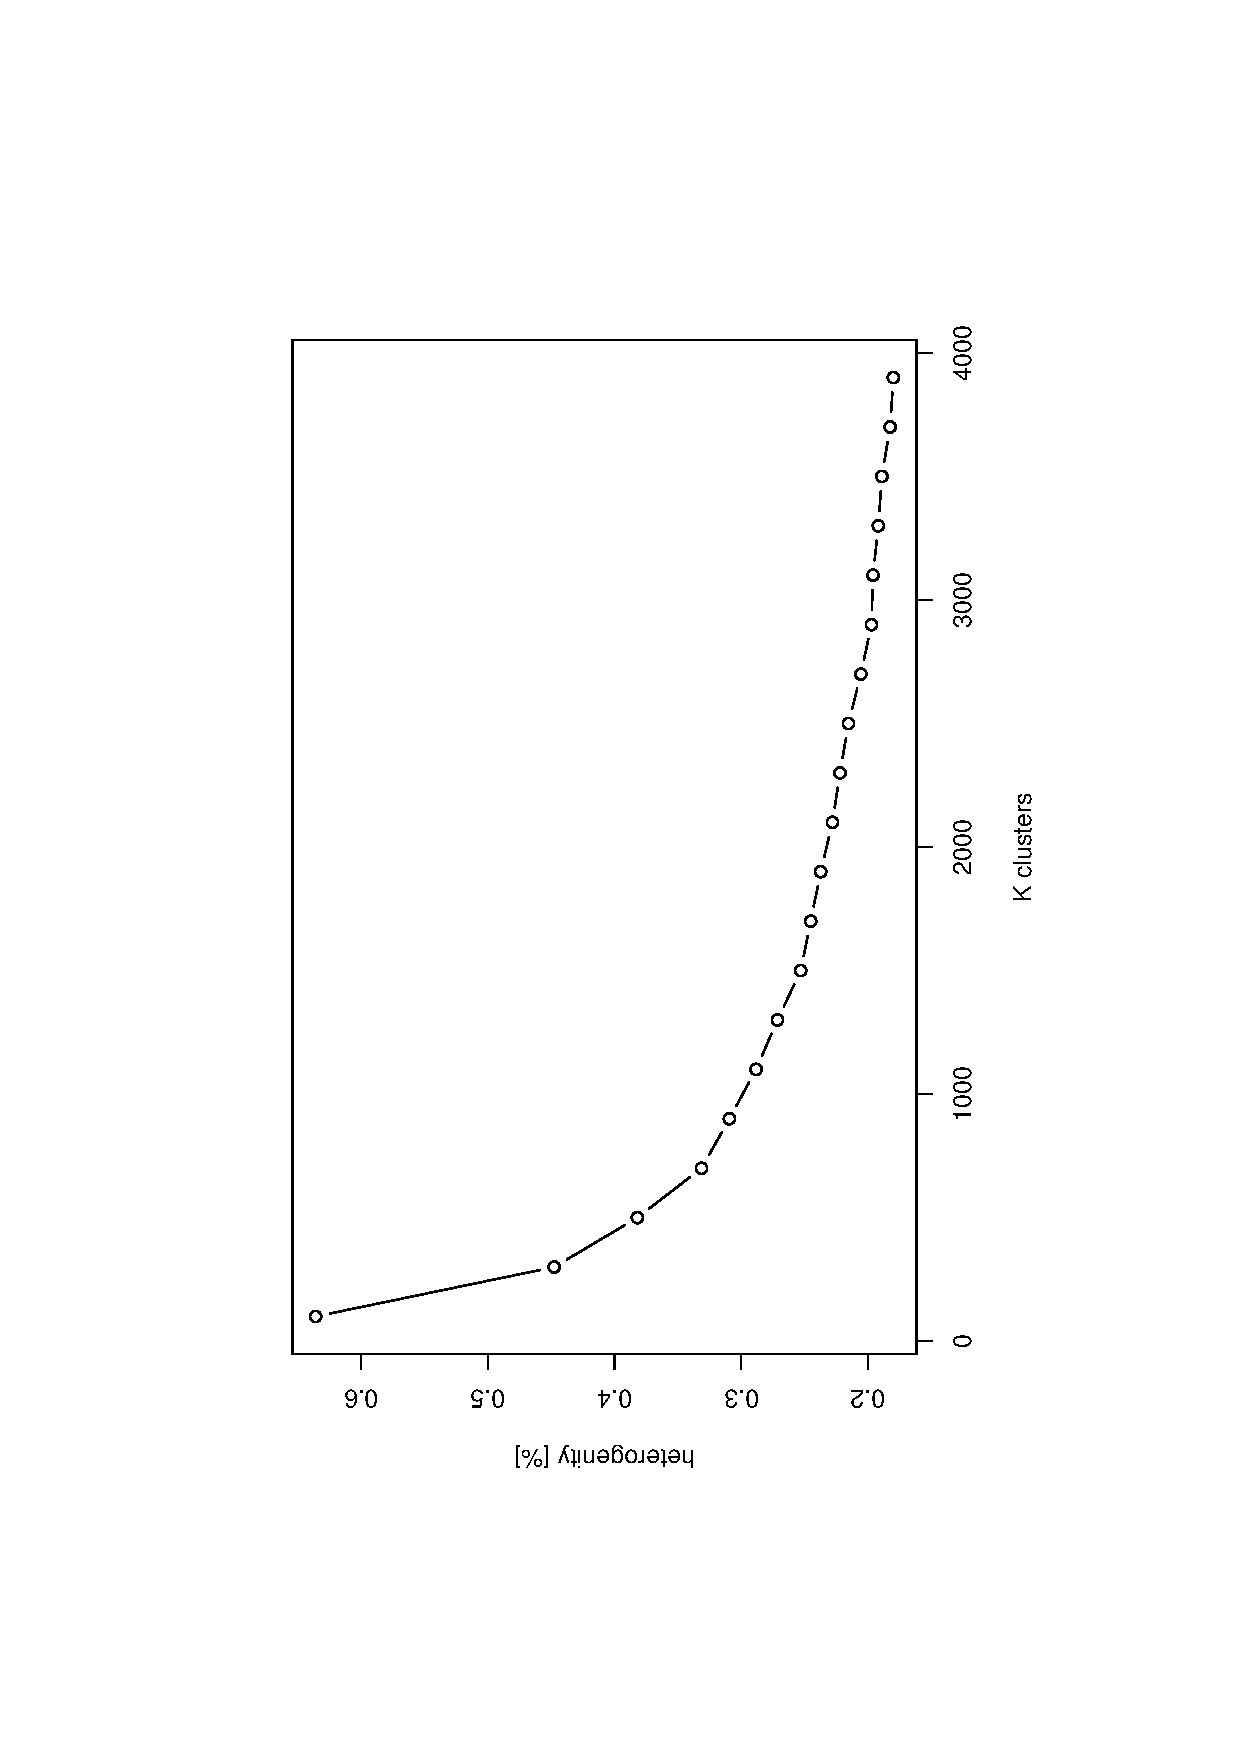
\includegraphics[width=\textwidth]{graphics/heterogenity}
\caption{Heterogeneity of the data set.}
\label{fig:heterogeneity_kmean}
\end{figure}

\begin{table}[H]
\centering
%# kmean = 400
%# k_knn = 10
%# k_mean = 10
%# kmean_iterations = 500
%# Time taken to prep kmean: 272.61"
%# [1] "Time taken to run kmean classification: 8.47000000000003"
%# [1] "Success for kmean: 0.4415"
%# [1] "Time taken to run raw knn classification: 1857.24"
%# [1] "Success for raw knn: 0.739"
\begin{tabular}{|l|r|r|}\hline
Criteria & Raw KNN & K-mean K-NN \\ \hline
Pre-Processing Time & 0s & 4m32.61s \\ \hline
Classification Time & 30m57.24s & 8.47s \\ \hline
Success Rate & 73.9\% & 44.2\% \\ \hline
\end{tabular}
\caption{Processing time comparison of running K-NN on K-mean data and raw}
\label{tab:processingtime_kmean_vs_raw_knn}
\end{table}

% \section{Decision Trees}

% \section{Introduction}

The classification of handwritten characters is used in a wide range of products to day.
Hence, this report goes in depth with how the numbers from zero to nine can be classified using machine learning algorithms.

The data set consists of a set of handwritten characters from zero to nine.
These were constructed by the students enrolled in the course Statistical Machine learning (RM-SML-E1) in 2015 at the University of Southern Denmark (SDU).
The characters were written in boxes of $0.55 \times 0.55 \textit{ cm}$ on a sheet with $20 \times 20$ boxes for each character.
The set used in this report is the 100DPI dataset.
Each number is hence stored as a $20 \times 20 \textit{ pixel}$ matrix containing the handwritten character.

The methods used for classification are K-Nearest Neighbours and Decision Trees.
This is to compare a method of lazy supervised learning against a method of supervised learning.
Furthermore a set of different ways to pre-process the data is explored.
Finally the two methods are compared with each at the best parameters and preprocessing settings.

The goal is to tests the handwritten digits from 20 people enrolled in the course.
The first test is where all people are mixed together, everybody contributing 90\% of their data to the training set and 10\% to the test set.
This is considered the easy problem as special ways of writing a digit will be represented in the training data.

Another test is to use 19 people's digits as training data and use the last person to test.
This is considered the hard problem.

To test the performance of the classification methods a simplified problem has been constructed.
It takes training data from a single person, Lukas Schwartz, which is referred to as Group 3 member 2 (G3M2).
By splitting the data 90\% for training and 10\% for testing
360 digits from each class as training data and 40 digits was used.
Testing each parameter with the simplified problem means the parameters could be tested in less time than if using the entire data set.

% \subsection{Entropy}
To compute the optimum decision point for the individual principle components, the entropy method is used.
The entropy of the PC's with our ten ciphers is given by equation \ref{eq:entropy}.

\begin{equation}
Entropy(S) = \sum_{i = '0'}^{'9'} -p_i \cdot \log_2(p_i) 
\qquad \because p_i = P(x = i)
\label{eq:entropy}
\end{equation}

To find the best decision point, it is wanted that the entropy of the two resulting systems, when dividing one PC into two, is as low as possible.
This can be represented as sum of entropy for our two resulting datasets, weighted by the relative size of such.
This is given in equation \ref{eq:entropy_datasetdevision}.

\begin{eqnarray}
Entropy = \sum_{i = 1}^{2} \frac{s_i \cdot Entropy(S_i)}{\sum_{k = 1}^{2} s_k} 
\qquad \because S_i \subset S\ and\ s_k = size(S_k)
\label{eq:entropy_datasetdevision}
\end{eqnarray}

When using equation \ref{eq:entropy_datasetdevision} on the first five principle components on the data of 15 people from the class, then figure \ref{fig:entropy_pc5} was gained.

\begin{figure}[H]
\centering
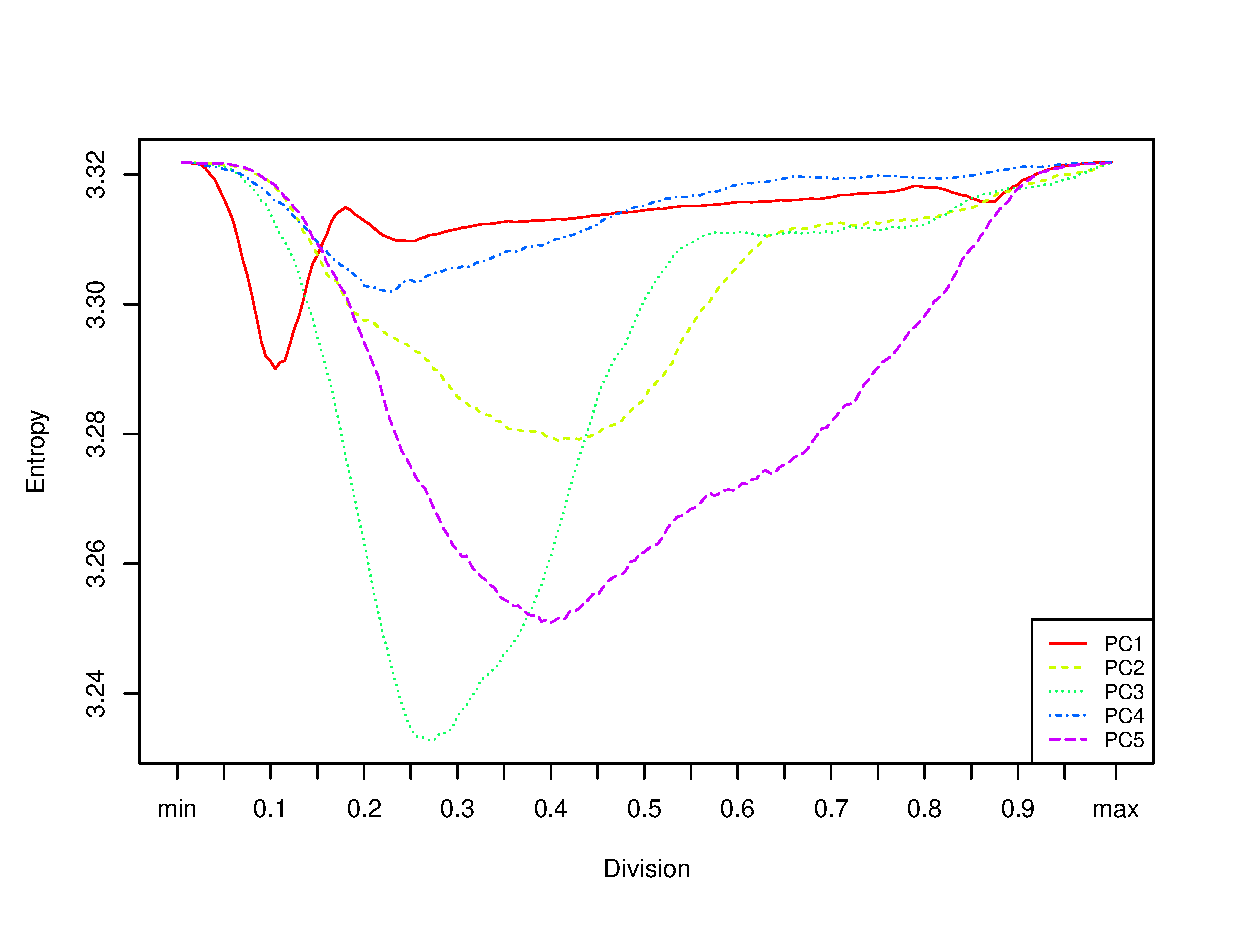
\includegraphics[width = 0.9 \textwidth]{graphics/entropy_pc}
\caption[Variation of the entropy]{Figure showing the variation of the entropy of the dataset when the decision point varies. Computed using equation \ref{eq:entropy_datasetdevision}. The data of the first five principle component.}
\label{fig:entropy_pc5}
\end{figure}


The point of lowest entropy for a principle component was then used as the splitting point to convert the data into binary.
This was done by setting everything below the splitting point to true and the rest false.
This was then done for all principle components on both the test and train set. 
The splitting point for the components in the test set were taken as the splitting point from the same component in the train set.

The optimal decision decision point is shown along with the PC values for PC1 in figure \ref{fig:decision_point}. 
The different data rows represent the ten different characters (from zero to nine).
Here it is clear that if the data is above the split then it is highly unlikely to be a 0.
If the data is below, further investigation is needed.
By removing all unlikely classes the true class must remain.

\begin{figure}[H]
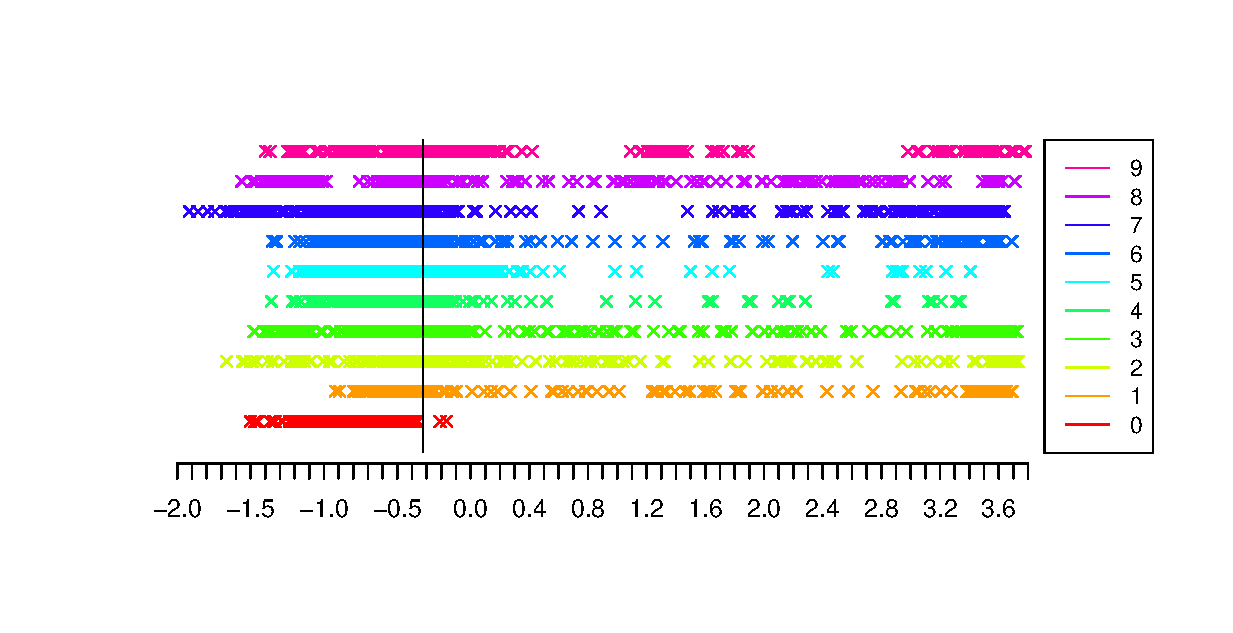
\includegraphics[width = \textwidth]{graphics/decision_seperation}
\caption{Decision point in relation to PC values.}
\label{fig:decision_point}
\end{figure}






% \subsection{Decision Trees}

\begin{figure}[H]
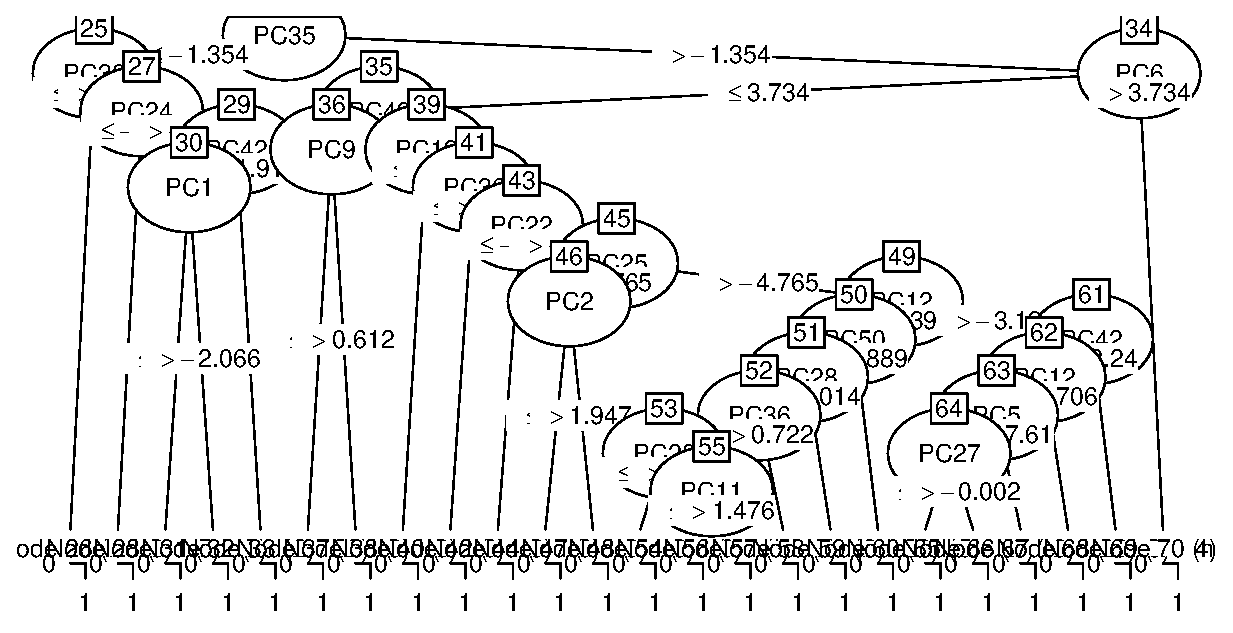
\includegraphics[width = \textwidth]{graphics/tree_section}
\end{figure}

\begin{figure}[H]
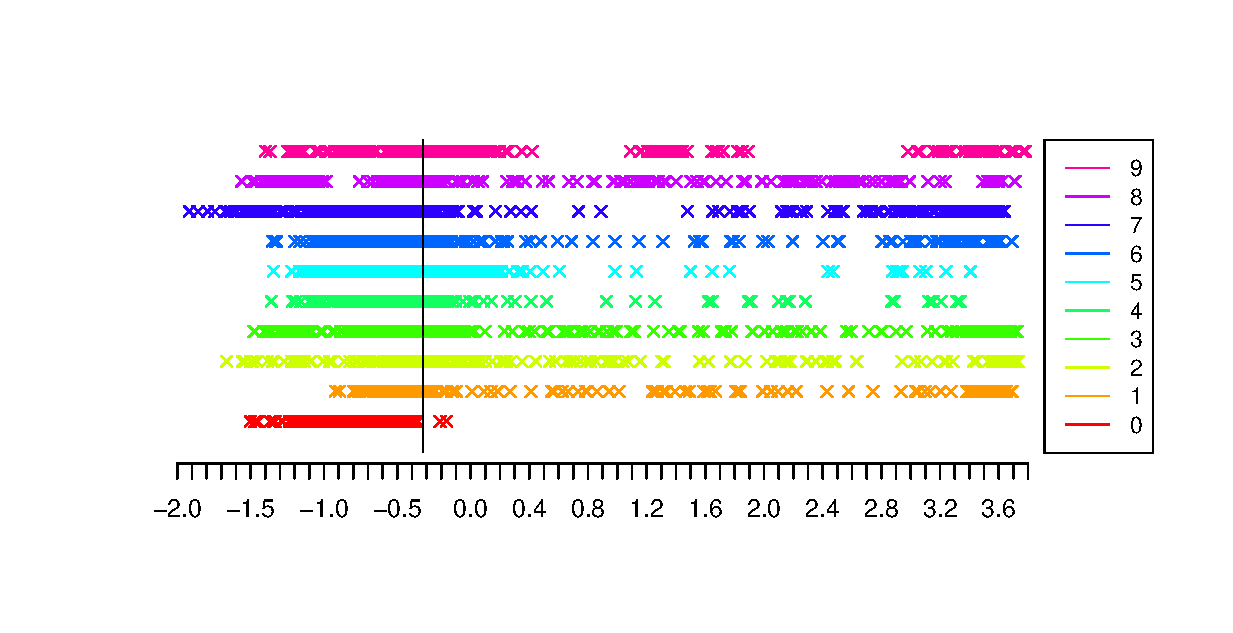
\includegraphics[width = \textwidth]{graphics/decision_seperation}
\end{figure}


\begin{table}[H]
\begin{tabular}{*{11}{c}}
&0	& 1	& 2	& 3	& 4	& 5	& 6	& 7	& 8	& 9 \\
\hline
0	& 250	& 19	& 13	& 12	& 13	& 34	& 53	& 16	& 31	& 19 \\
1	& 1	& 235	& 24	& 22	& 7	& 16	& 6	& 23	& 7	& 22 \\
2	& 19	& 12	& 179	& 36	& 3	& 9	& 15	& 39	& 48	& 19 \\
3	& 18	& 7	& 17	& 119	& 9	& 31	& 31	& 59	& 37	& 28 \\
4	& 8	& 15	& 23	& 21	& 205	& 18	& 28	& 32	& 14	& 79 \\
5	& 27	& 23	& 10	& 59	& 15	& 192	& 30	& 12	& 36	& 17 \\
6	& 36	& 62	& 41	& 28	& 3	& 33	& 194	& 7	& 28	& 31 \\
7	& 9	& 2	& 16	& 7	& 64	& 6	& 3	& 161	& 15	& 21 \\
8	& 26	& 17	& 70	& 73	& 4	& 54	& 34	& 22	& 151	& 25 \\
9	& 6	& 8	& 7	& 23	& 77	& 7	& 6	& 29	& 33	& 139 \\

\end{tabular}

\end{table}

% \subsection{Random Forests}

A random forest was computed in figure \ref{fig:success_time_vs_trees_randomForest} using G3M2 data as test set and the remaining 15 students as train set.
The number of trees was varied and the time measured.

\begin{figure}[H]
\centering
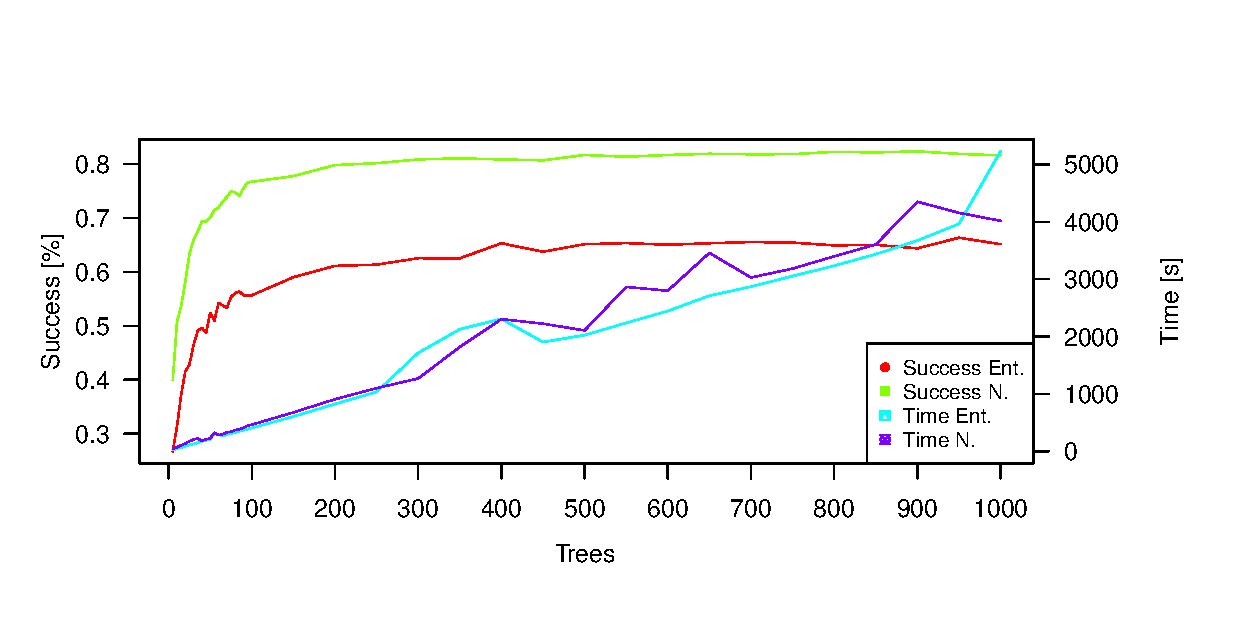
\includegraphics[width = 0.95 \textwidth]{graphics/successRate_randomForest}
\caption{Success rate and time taken to compute the trees needed in the random forest as the number of trees increases.}
\label{fig:success_time_vs_trees_randomForest}
\end{figure}

As can be seen on figure \ref{fig:success_time_vs_trees_randomForest}, then the success rate increases drastically from 0 to 500 trees in the random forest where it settles at around 70\%.
The time increases exponentially with the number of trees.

From figure \ref{fig:success_time_vs_trees_randomForest} it was decided to use 700 trees for the optimum random forest.
Figure ... was generated using the 700 trees.
Each point was computed using 


\Huge{Make comparison of all with best forest settings.}

%\section{Naive Bayes}
%\section{Introduction}

The classification of handwritten characters is used in a wide range of products to day.
Hence, this report goes in depth with how the numbers from zero to nine can be classified using machine learning algorithms.

The data set consists of a set of handwritten characters from zero to nine.
These were constructed by the students enrolled in the course Statistical Machine learning (RM-SML-E1) in 2015 at the University of Southern Denmark (SDU).
The characters were written in boxes of $0.55 \times 0.55 \textit{ cm}$ on a sheet with $20 \times 20$ boxes for each character.
The set used in this report is the 100DPI dataset.
Each number is hence stored as a $20 \times 20 \textit{ pixel}$ matrix containing the handwritten character.

The methods used for classification are K-Nearest Neighbours and Decision Trees.
This is to compare a method of lazy supervised learning against a method of supervised learning.
Furthermore a set of different ways to pre-process the data is explored.
Finally the two methods are compared with each at the best parameters and preprocessing settings.

The goal is to tests the handwritten digits from 20 people enrolled in the course.
The first test is where all people are mixed together, everybody contributing 90\% of their data to the training set and 10\% to the test set.
This is considered the easy problem as special ways of writing a digit will be represented in the training data.

Another test is to use 19 people's digits as training data and use the last person to test.
This is considered the hard problem.

To test the performance of the classification methods a simplified problem has been constructed.
It takes training data from a single person, Lukas Schwartz, which is referred to as Group 3 member 2 (G3M2).
By splitting the data 90\% for training and 10\% for testing
360 digits from each class as training data and 40 digits was used.
Testing each parameter with the simplified problem means the parameters could be tested in less time than if using the entire data set.

%
%\subsection{Data Normalization}
\label{sec:DataNormalization}
When comparing multiple entries in a dataset, it might be beneficial to normalize such to obtain a basis for equal comparison.
In the case of numbers being written and detected, such as ours, there might be differences in the colors of the characters when different pens/pencils are used.
This can create unwanted differences between elements in a category, which are else identically, and hence lead to false predictions.
Two normalization algorithms where hence implemented.
These are, min-max normalization and z-score standardization.

Figure \ref{fig:normalization_test_pre-post} shows the result when cross validation is carried out on the data from the 16 people in the class.
In figure \ref{fig:normalization_test_pre-post}, each individual is tested up against the rest of the group without contributing to the training set themselves. 
The two types of normalization are performed both before and after the data reduction using PCA.


\begin{figure}[H]
\centering
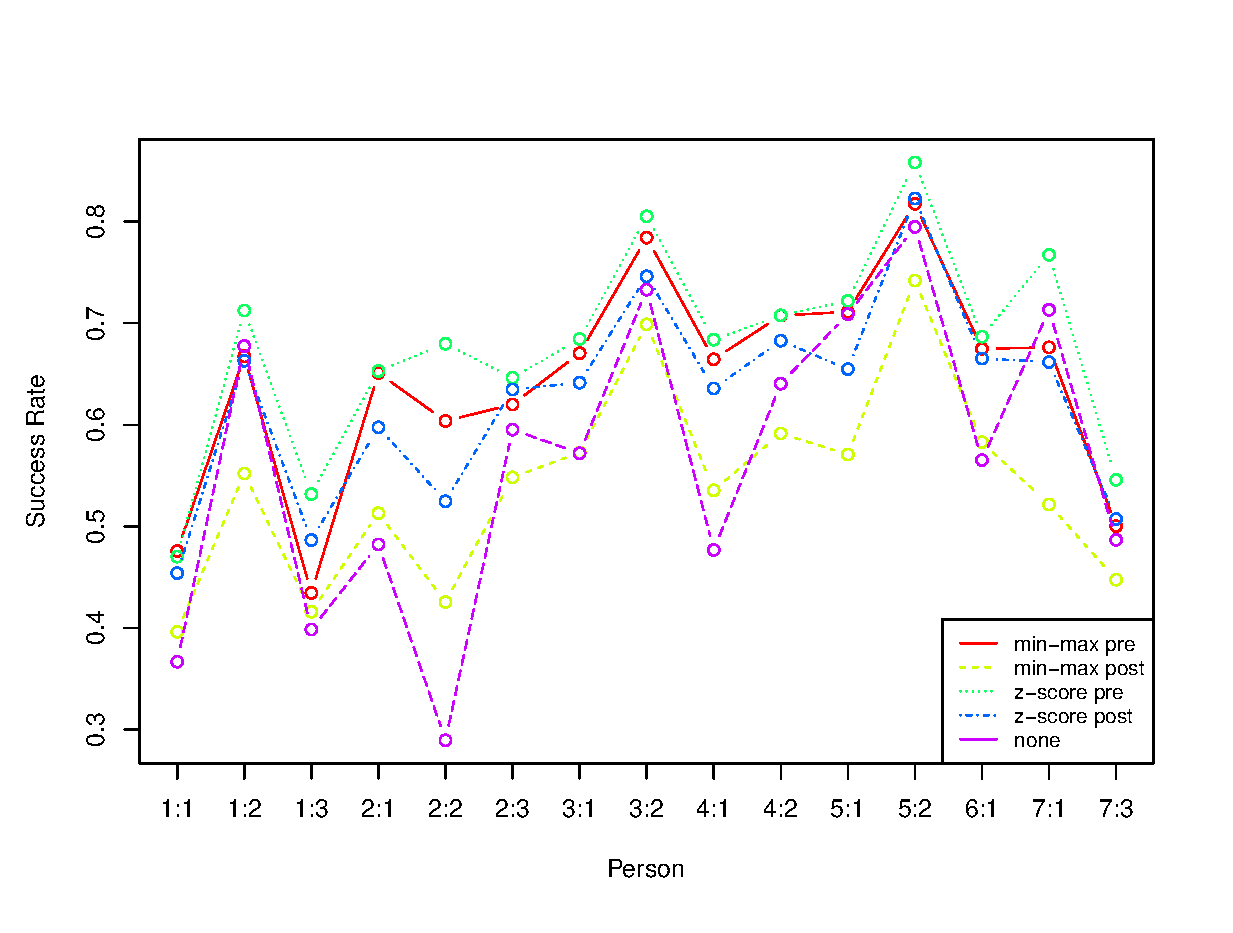
\includegraphics[width = \textwidth]{graphics/graph_normalization}
\caption[Comparison of different students.]{Success rate for detection of characters of on person when not in the training set. 
Data normalized before (pre) and after (post) dataset reduction using PCA.
PCA was set to ensure that 80\% of all variance was included in the data set and K as 10.
The person tested for is given as 'Group':'Member'.
It was tested with 16 people.}
\label{fig:normalization_test_pre-post}
\end{figure}

The mean success rate of figure \ref{fig:normalization_test_pre-post} is listed in table \ref{tab:meanSuccess_normalization_test_pre-post}.
From both the graph and table, it can be concluded that the z-score standardization before the PCA reduction performs, on average, at least 3\% better than the other methods.

The figure \ref{fig:normalization_test_pre-post} also shows that in general all three normalizations, except for the min-max normalization after PCA reduction, is on average, yielding a higher number of correct predictions.

The normalization before the PCA reductions yields a better result in all cases. 
This may be because it enables the PCA to find the features being more responsible for the decision of which category a element belongs to. 
Some of the performance improvement can be because of features of a low variance in their measured value, have a larger relevance as to what the actual category of the elements are.

\textbf{UPDATE TABLE!}

\begin{table}[H]
\centering
\begin{tabular}{|l|r|}\hline
% 0.5720167 0.4639500 0.6055167 0.5521333 0.5034333
Normalization Method & Mean Success \\ \hline
Min-Max Normalization Pre & 57.2 \% \\ \hline
Min-Max Normalization Post & 46.4 \% \\ \hline
Z-Score Normalization Pre & 60.6 \% \\ \hline
Z-Score Normalization Post & 55.2  \% \\ \hline
No Normalization & 50.3 \% \\ \hline
\end{tabular}
\caption{Mean success rates for normalization test as seen in figure \ref{fig:normalization_test_pre-post}.}
\label{tab:meanSuccess_normalization_test_pre-post}
\end{table}



\subsubsection{Performance Effect when adding a Filter}

\begin{figure}[H]
\centering
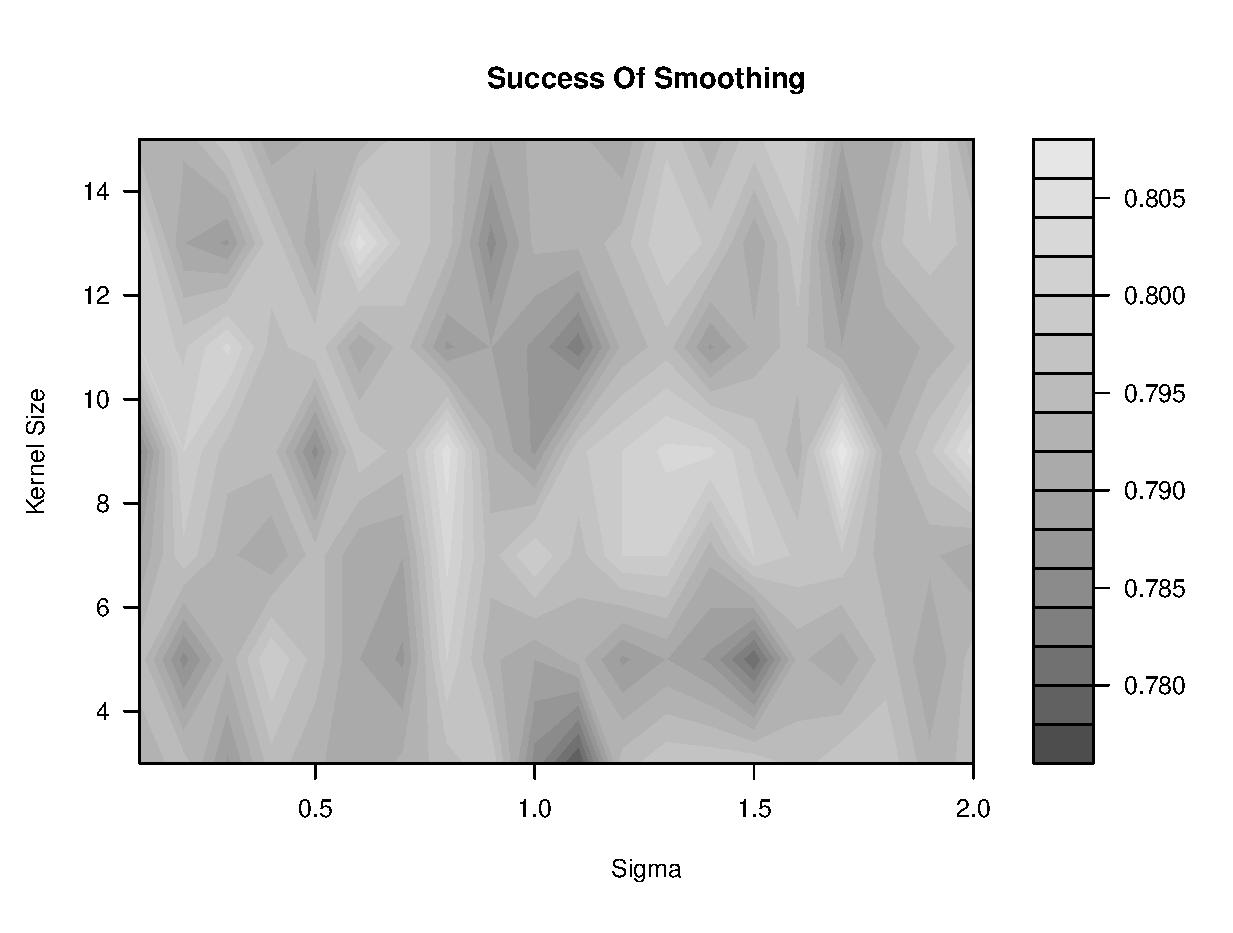
\includegraphics[width = \textwidth]{graphics/success_of_smoothing_contour}
\caption[Optimal smoothing]{Impact of sigma and kernel size when smoothing an image. 
Tested with group 3 member 2's data against 14 other students.
}
\label{fig:smoothing_contour}
\end{figure}

To find the optimal kernel size the success detection rate was plotted with a varying $\sigma$. 
The optimal kernel size is chosen to be 9 pixels wide.
From figure \ref{fig:smoothing_contour} it is concluded that a filter size of 9 is optimal.

Using this knowledge figure \ref{fig:normalization_test_with_smooth} was generated.
The figure compares the unprocessed success rate compared to that of the z-score pre and z-score pre with gaussian smoothing (filter size 9 and sigma 0.7).

 \begin{figure}[H]
 \centering
 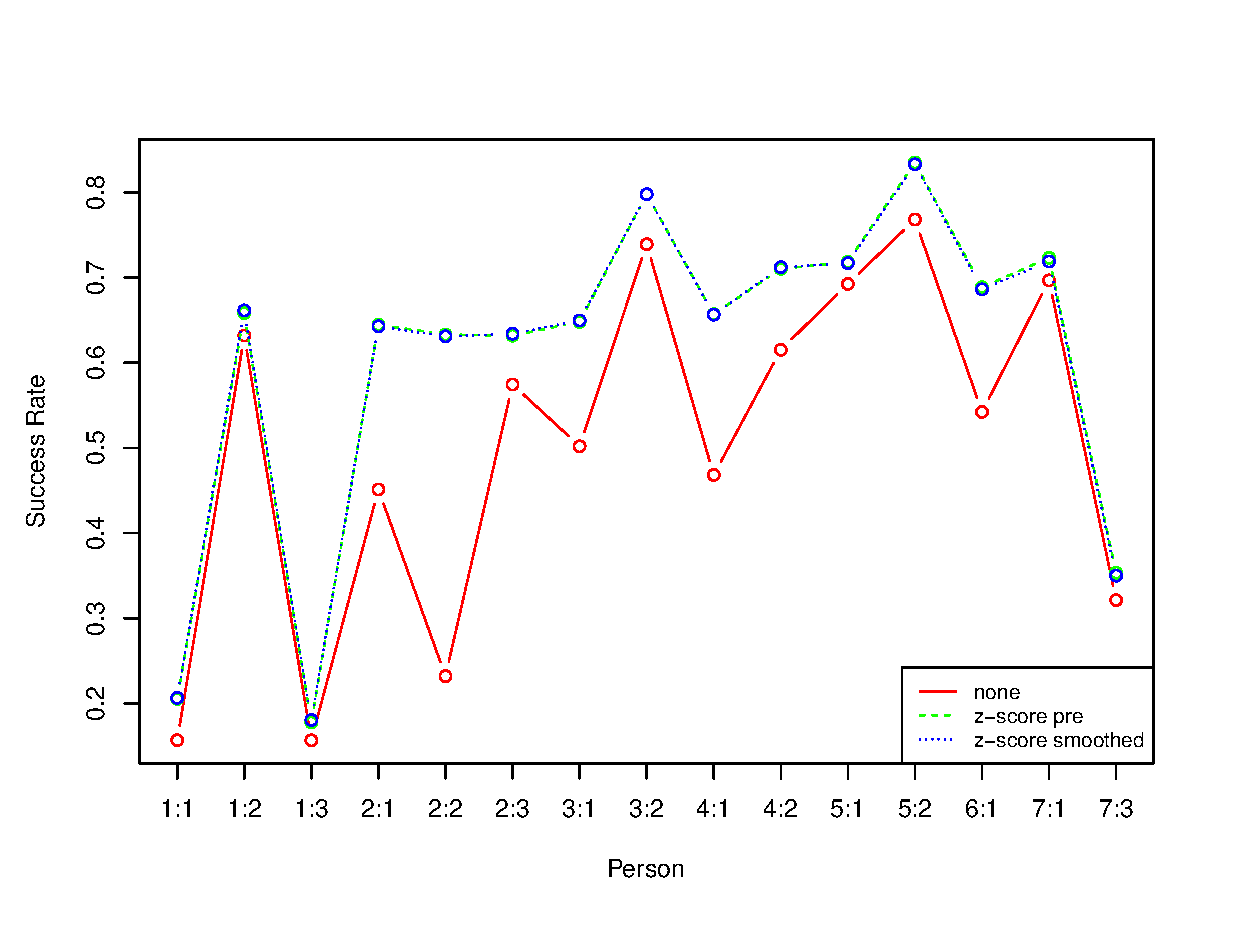
\includegraphics[width = \textwidth]{graphics/graph_normalization_smoothed}
 \caption[Filtered and normalized data.]{Filtered data normalized vs unfiltered normalized data.
 Running each person against the rest of the class in the train set.
 }
 \label{fig:normalization_test_with_smooth}
 \end{figure}

As seen on figure \ref{fig:normalization_test_with_smooth}, then the result of smoothing the data before normalization is not improving the data.

%
%\subsection{Naive Bayes Comparison of Methods}
In order to find the best of the two methods discussed earlier for the classification of handwritten digits, the two methods are compared.
This is done by varying their key parameters and see how this affects the success.

\subsubsection{Pixel Binning}
To find one of the the best settings for the Naive Bayes, a contour for the number of bins and the accumulated variance in the PCA analysis was made.

\begin{figure}[H]
\centering
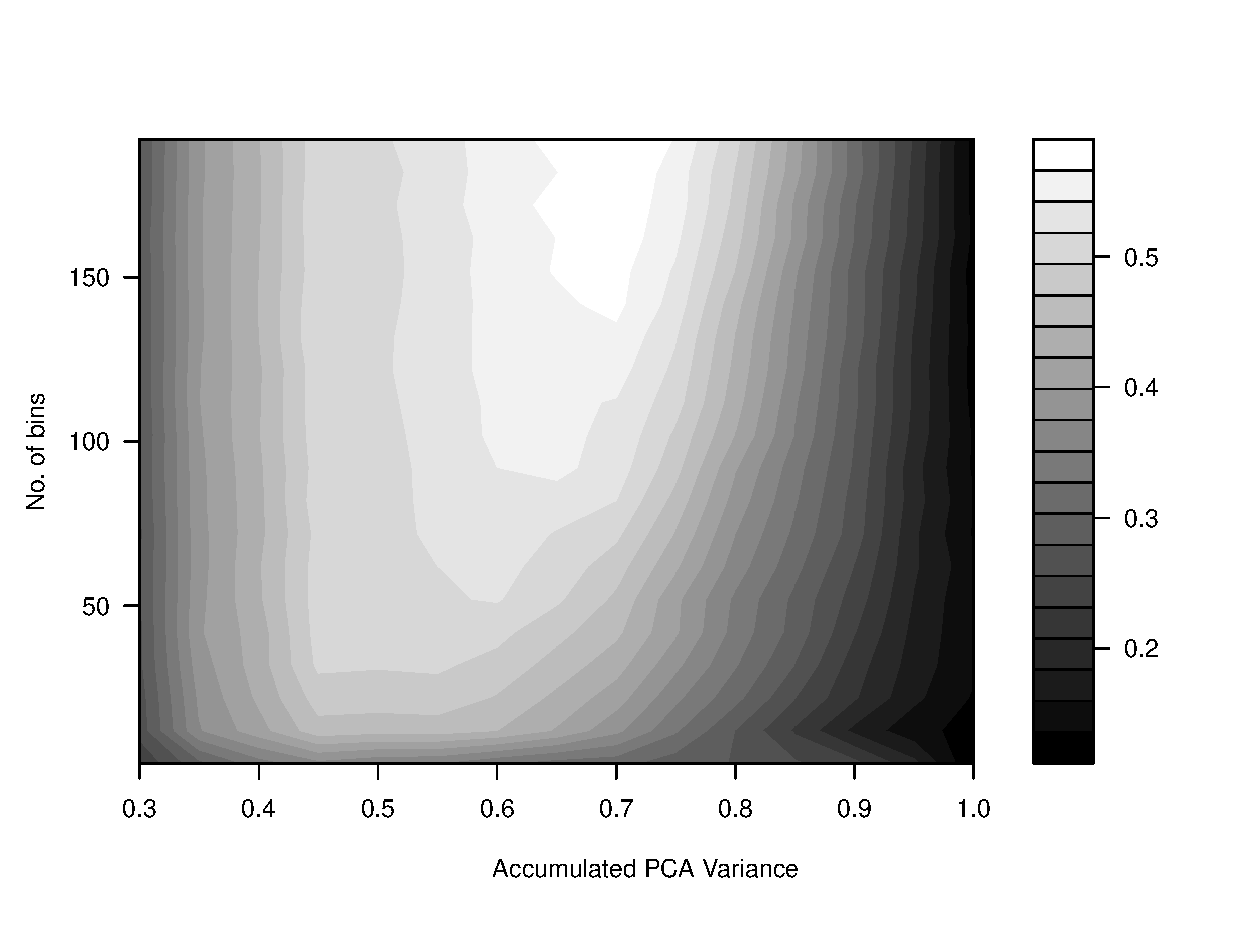
\includegraphics[width = \textwidth]{graphics/contour_bins_vs_pca}
\caption{Contour of the success rate of the Naive Bayes with accumulated PCA going from 0.3 to 1 and the number of bins from 2 to 192.
The data was normalized using z-score first and the Laplace value was set to 1.
The contour was created with G3M2's data in the test set and the remaining 15 loadable datasets in the training set.}
\label{fig:contour_bin-vs-pca}
\end{figure}

From figure \ref{fig:contour_bin-vs-pca} it can be seen that the best point goes out of the view, and is in fact increasing, indicating that it gets better the higher dimensional the data is. The best bin size can hence not be determined. The most optimum point would be around 40 bins and an accumulative PCA of 50\% as at this point, the increase PCA and bins does not improve the success by an considerably enough compared to how much the timing would increase.

The Laplace value of the Naive Bayes was also tested, but due to unknown reasons, then the Laplace coefficient did not have any effect on the success of the method.
It was therefore decided not to show the effect of such in this report.

\subsubsection{Pixel Bin Occurrence}
A contour of the number of bins used to represent a pixel and the number of horizontal stripes the image is divided into is shown in figure \ref{fig:contour_bin-vs-div}.

\begin{figure}[H]
\centering
%\includegraphics[width = \textwidth]{graphics/contour_bins_vs_div}
\caption{Contour of the success rate of the Naive Bayes with the number of bins used to represent a pixel and the number of horizontal stripes the image is divided into.
The contour was created with G3M2's data in the test set and the remaining 15 loadable datasets in the training set.}
\label{fig:contour_bin-vs-div}
\end{figure}

It can be seen on figure \ref{fig:contour_bin-vs-div} that ... graph to be seen...



\subsubsection{Selection of the Methods}
Comparing the two graphs in figure \ref{fig:contour_bin-vs-pca} and \ref{fig:contour_bin-vs-div} it can clearly be seen that the first method used for figure \ref{fig:contour_bin-vs-pca} performs considerably better than the other method proposed.
It was therefore decided only to continue with the better method.

%
%\subsection{Naive Bayes Optimization}

The timing was measured with different bin sizes. 
In figure \ref{fig:baye_timing} the timing and success can be seen.
The timing is linear and there is no increase in successful classifications with more than 100 bins. 
The time it took to normalize the data into bins and calculate the naive Bayes is shown.

\begin{figure}[H]
\centering
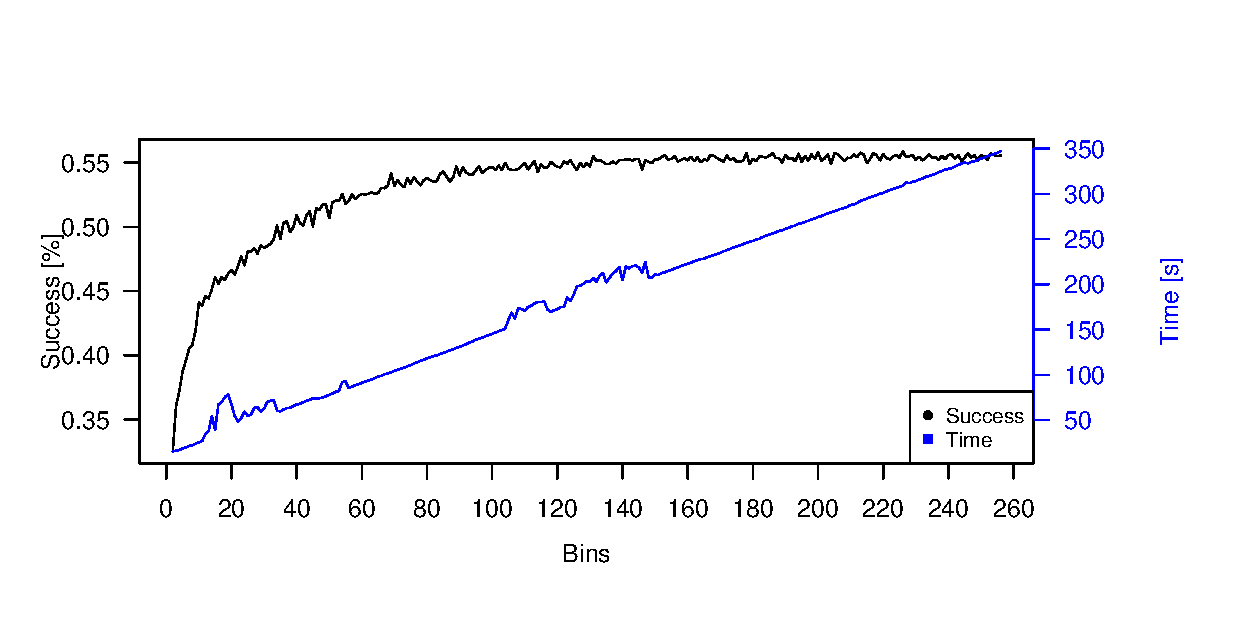
\includegraphics[width = \textwidth]{graphics/baye_timing_bins}
\caption[Timing with different bin sizes]{Timing and success of different bin sizes. Data was tested on Group 3 member 2's data vs 16 people.}
\label{fig:baye_timing}
\end{figure}


The best values for bins and PCA are taken from figure \ref{fig:contour_bin-vs-pca} and then used to compare every person with the rest of the class as seen in figure \ref{fig:comp_naiveBayes}.

\begin{figure}[H]
\centering
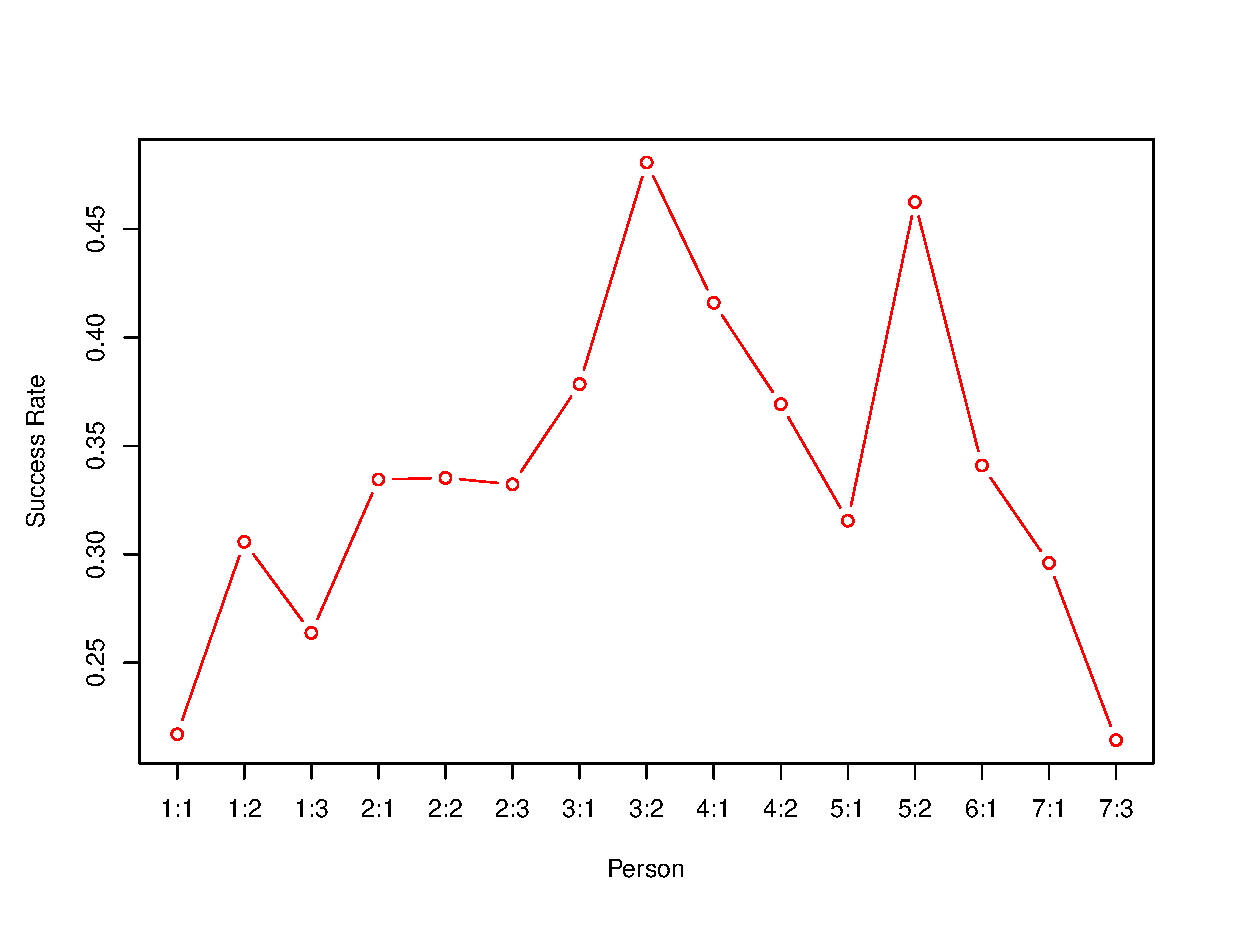
\includegraphics[width = \textwidth]{graphics/graph_baye_comparison}
\caption{Comparison of Naive Bayes for one person with the rest of the class.
Where bins is 50 and PCA is 50\%. The mean success rate is 34.6\%.}
\label{fig:comp_naiveBayes}
\end{figure}

From here it can be seen that this method performs rather bad when testing on the whole class.
With a mean success of 34.6\% for the Naive Bayes, the chance of detecting a decimal correctly is considerably worse than any other previous method  encountered and hence not recommended.

A confusion matrix is also given in table \ref{tb:confus_bayes}.
This is made under same circumstances as figure \ref{fig:comp_naiveBayes} with the test person set to G3M2.

\begin{table}[H]
\centering
	\begin{subtable}{0.75\textwidth}
        \centering
        
\begin{tikzpicture}
            \node at (0,0) {\Large Actual Class}; 
        \end{tikzpicture}
    \end{subtable}
    
    \begin{subtable}{0.05\textwidth}
        \flushright
        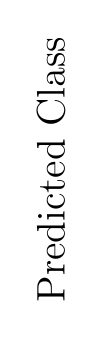
\begin{tikzpicture}
            \node[rotate=90] {\Large Predicted Class};
        \end{tikzpicture}
    \end{subtable}
    \begin{subtable}{0.7\textwidth}
            \centering
%            {\scriptsize
                \begin{tabular}{l|*{10}{c}}
                    &0	& 1	& 2	& 3	& 4	& 5	& 6	& 7	& 8	& 9 \\
\hline
0	& 311	& 8	& 17	& 0	& 1	& 57	& 15	& 13	& 4	& 4 \\
1	& 13	& 247	& 58	& 19	& 19	& 17	& 9	& 37	& 33	& 41 \\
2	& 7	& 5	& 116	& 8	& 0	& 5	& 14	& 32	& 33	& 0 \\
3	& 2	& 18	& 3	& 106	& 0	& 2	& 11	& 50	& 22	& 3 \\
4	& 15	& 15	& 12	& 26	& 323	& 37	& 47	& 92	& 3	& 73 \\
5	& 8	& 4	& 3	& 16	& 0	& 81	& 2	& 0	& 10	& 10 \\
6	& 12	& 38	& 76	& 42	& 5	& 98	& 260	& 5	& 39	& 9 \\
7	& 0	& 1	& 1	& 2	& 0	& 10	& 0	& 109	& 1	& 0 \\
8	& 25	& 45	& 111	& 150	& 0	& 59	& 27	& 15	& 218	& 11 \\
9	& 7	& 19	& 3	& 31	& 52	& 34	& 15	& 47	& 37	& 249 \\

                \end{tabular}
%            }
    \end{subtable}
    \caption{Confusion matrix for Naive Bayes.
    Where bins is 50 and PCA is 50\%. The total success is 50.5\%.}
    \label{tb:confus_bayes}
\end{table}

The data from the confusion matrix in table \ref{tb:confus_bayes} is used to group the ten different decimals into three different groups depending on how well they are detected.
These are seen in table \ref{tab:dec_eval_confus}.

\begin{table}[H]
\centering
\begin{tabular}{|l|c|}
\hline
Group & Decimal \\ \hline
Good ($\geq$ 75\%) & 0, 4 \\ \hline
Intermediate (50\% to 75\%) & 1, 6, 8, 9 \\ \hline
Bad ($\leq$ 50\%) & 2, 3, 5, 7 \\ \hline
\end{tabular}
\caption{Decimal evaluation of confusion matrix in table \ref{tb:confus_bayes}.}
\label{tab:dec_eval_confus}
\end{table}

As can be seen in table \ref{tab:dec_eval_confus}, then the detection of 0 and 4 is quite good, but there is a large amount of miss detected numbers.
The 2's and 3's are often confused with the 8 and the 5 is in many cases confused with the 6.
It can furthermore be seen that the classes 5 and 7 are rarely used to describe a prediction.
Why this is so could be due to their close resemblance to the other classes such as 6 in the case of 5.
%
%\subsection{Kernel Density Estimation}

Kernel density estimation (KDE) is a method that derives a density plot from training data.
If the data is reduced to a sum of the pixel values each training set could be used to estimate the probability that a sum occurs given a specific classification. 
We could denote this as \(P(x|c)\) where x is the sum we want to compare and c is the classification.
We want to be able to turn this into \(P(c|x)\) and with Bayes formula this is possible. 
\[P(c|x) = \frac{P(x|c) \cdot P(c)}{P(x)}\]
So by making a density function for each \(P(x|c)\) the problem can be reduced to comparing a density function for each class and selecting most likely.

In figure \ref{fig:pdf_sum_kde} these density functions can be seen. 
Since the data has been reduced to a single data point the density plots overlap. 
The density plots that rise above the others will always be chosen so this is not a good way to do this.

\begin{figure}[H]
    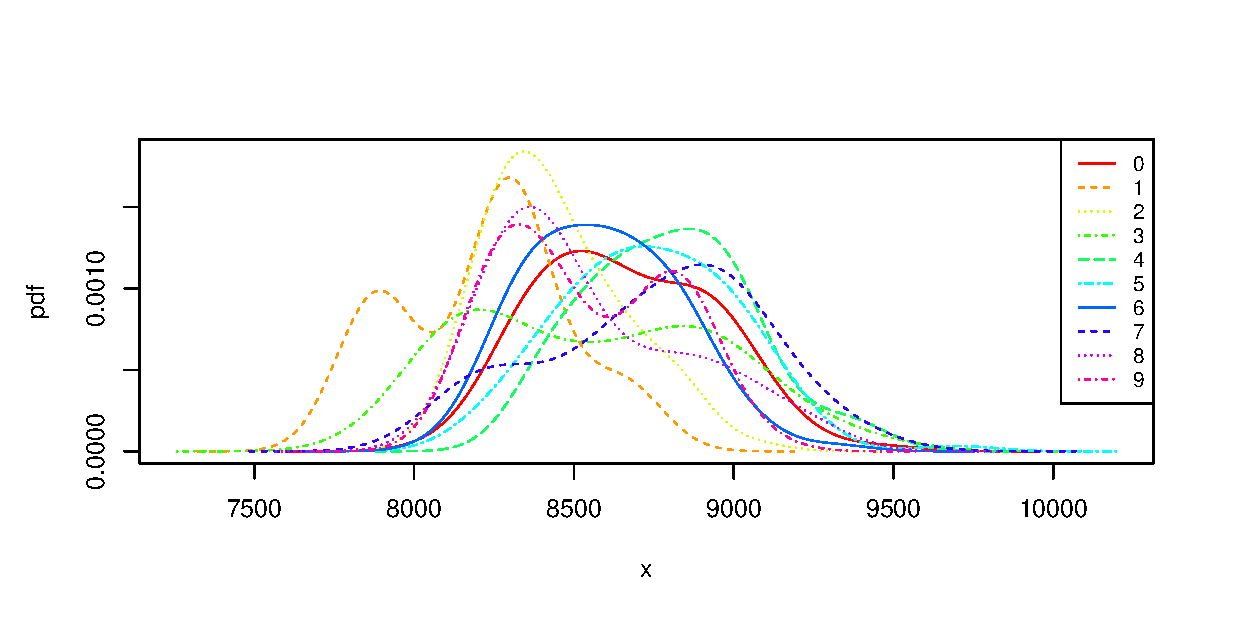
\includegraphics[width = \textwidth]{graphics/kde_graphs_sum}
    \caption{Density plot for each classification. The sum of all pixels are compared.}
    \label{fig:pdf_sum_kde}
\end{figure}

To see if it was possible to differentiate the data without increasing the dimensions, different summation techniques were tried. 
In figure \ref{fig:pdf_gaussian_kde} a Gaussian sum was compared. Weighting the data closest to the center higher than the data far away gave a different result although the data still overlaps.
In table \ref{tb:kde_confus} the classifications is displayed. 
If a better way to differentiate the data is used it could be useful to test as the data it was able to detect had above 48\% successful detections.

\begin{figure}[H]
    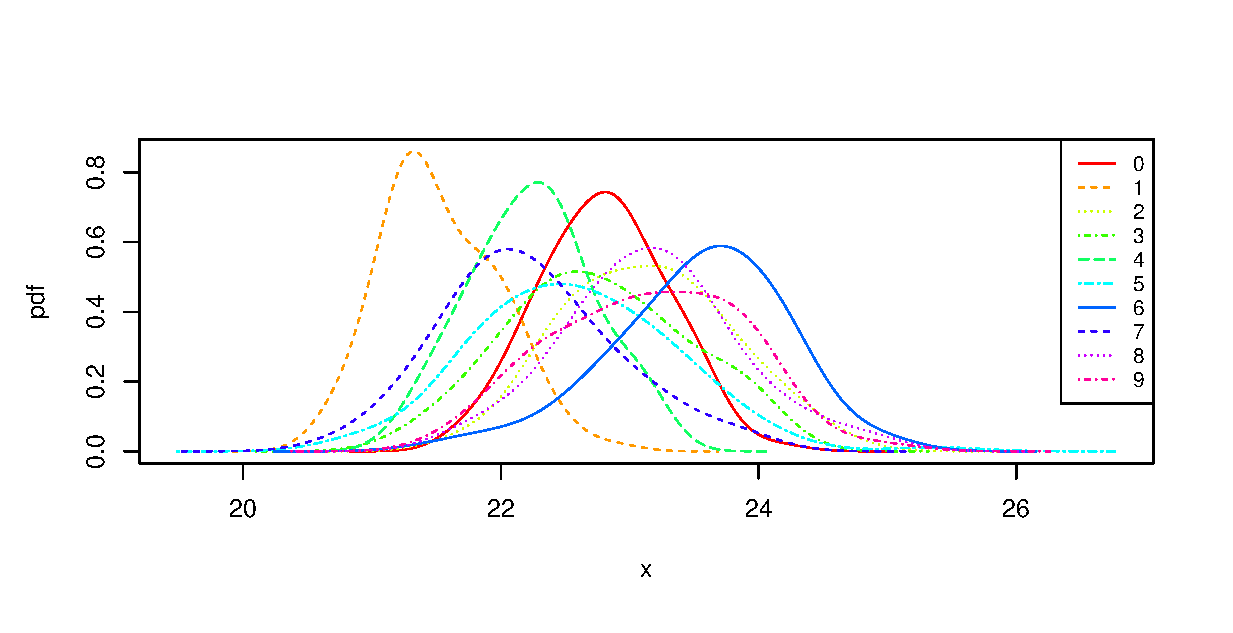
\includegraphics[width = \textwidth]{graphics/kde_graphs}
    \caption{Density plot for each classification. A Gaussian sum was compared.}
    \label{fig:pdf_gaussian_kde}
\end{figure}

\begin{table}[H]
\centering
         \begin{subtable}{0.75\textwidth}
        \centering
        
\begin{tikzpicture}
            \node at (0,0) {\Large Actual Class}; 
        \end{tikzpicture}
    \end{subtable}
    
    \begin{subtable}{0.05\textwidth}
        \flushright
        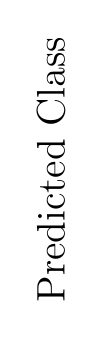
\begin{tikzpicture}
            \node[rotate=90] {\Large Predicted Class};
        \end{tikzpicture}
    \end{subtable}
    \begin{subtable}{0.7\textwidth}
            \centering
%            {\scriptsize
                \begin{tabular}{l|*{10}{c}}
                    &0	& 1	& 2	& 3	& 4	& 5	& 6	& 7	& 8	& 9 \\
\hline
0	& 0	& 0	& 0	& 0	& 0	& 0	& 0	& 0	& 0	& 0 \\
1	& 0	& 41	& 1	& 3	& 0	& 0	& 0	& 0	& 0	& 3 \\
2	& 26	& 53	& 19	& 13	& 25	& 28	& 18	& 5	& 7	& 30 \\
3	& 0	& 0	& 0	& 3	& 0	& 0	& 1	& 1	& 0	& 1 \\
4	& 34	& 2	& 41	& 37	& 41	& 31	& 39	& 51	& 49	& 23 \\
5	& 0	& 0	& 2	& 1	& 0	& 0	& 4	& 2	& 1	& 1 \\
6	& 31	& 4	& 29	& 18	& 11	& 19	& 19	& 4	& 14	& 22 \\
7	& 9	& 0	& 8	& 25	& 23	& 22	& 19	& 37	& 29	& 20 \\
8	& 0	& 0	& 0	& 0	& 0	& 0	& 0	& 0	& 0	& 0 \\
9	& 0	& 0	& 0	& 0	& 0	& 0	& 0	& 0	& 0	& 0 \\

                    \multicolumn{11}{l}{\bf Success}\\
                    \multicolumn{1}{l}{}&0.49&0.48&0.00&0.00&0.55&0.00&0.82&0.00&0.04&0.00\\
                \end{tabular}
%            }
    \end{subtable}
    \caption{Confusion matrix for KDE.}
    \label{tb:kde_confus}
\end{table}


% \section{Neural Networks and Support Vector Machines}
% \section{Introduction}

The classification of handwritten characters is used in a wide range of products to day.
Hence, this report goes in depth with how the numbers from zero to nine can be classified using machine learning algorithms.

The data set consists of a set of handwritten characters from zero to nine.
These were constructed by the students enrolled in the course Statistical Machine learning (RM-SML-E1) in 2015 at the University of Southern Denmark (SDU).
The characters were written in boxes of $0.55 \times 0.55 \textit{ cm}$ on a sheet with $20 \times 20$ boxes for each character.
The set used in this report is the 100DPI dataset.
Each number is hence stored as a $20 \times 20 \textit{ pixel}$ matrix containing the handwritten character.

The methods used for classification are K-Nearest Neighbours and Decision Trees.
This is to compare a method of lazy supervised learning against a method of supervised learning.
Furthermore a set of different ways to pre-process the data is explored.
Finally the two methods are compared with each at the best parameters and preprocessing settings.

The goal is to tests the handwritten digits from 20 people enrolled in the course.
The first test is where all people are mixed together, everybody contributing 90\% of their data to the training set and 10\% to the test set.
This is considered the easy problem as special ways of writing a digit will be represented in the training data.

Another test is to use 19 people's digits as training data and use the last person to test.
This is considered the hard problem.

To test the performance of the classification methods a simplified problem has been constructed.
It takes training data from a single person, Lukas Schwartz, which is referred to as Group 3 member 2 (G3M2).
By splitting the data 90\% for training and 10\% for testing
360 digits from each class as training data and 40 digits was used.
Testing each parameter with the simplified problem means the parameters could be tested in less time than if using the entire data set.


% \subsection{Neural Networks}

Neural networks is a model based on biology. 
Initially all neurons are connected. 
When the connection is active the synapses becomes stronger and when the connection is inactive the synapses becomes weaker.

The Stuttgart Neural Network Simulator is implemented in R in the RSNNS package.
The package can make a model of a artificial neural network (ANN) as a multi-layered perceptron.
To reduce the inputs the data is normalized using the Z-Score method and a principle components analysis is made to give the most important data points.

\begin{figure}[h]
    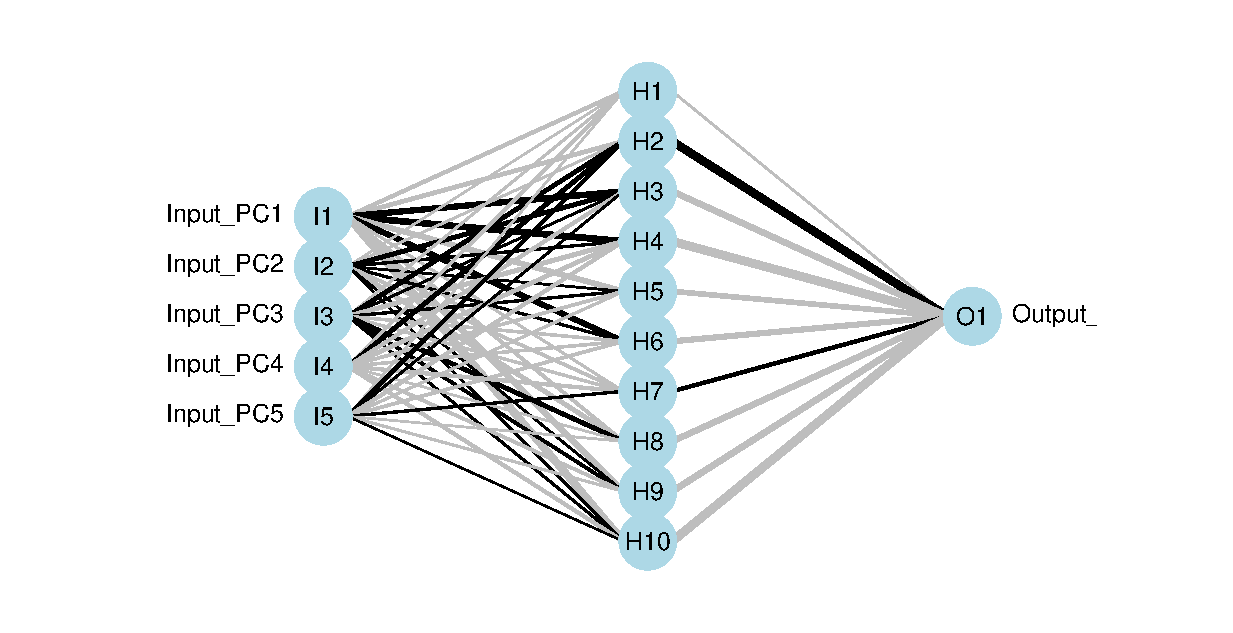
\includegraphics[width=\textwidth]{graphics/neural_network_visualized}
    \caption[Visualization of a ANN model.]{Visualization of a ANN model with 5 PC and 10 hidden layers. Plotted using \url{https://github.com/fawda123/NeuralNetTools}}
    \label{fig:neural_network_visualised}
\end{figure}

In the following section will the relationship with number of PC and the number of hidden layers be explored.
In figure \ref{fig:neural_network_visualised} is a small ANS shown.
The thickness of the synapses indicates the weight.
The black color indicates a positive weight and the grey color indicates a negative weights.
It is important to notice that there is only a single output. 
Testing a digit will only show if the entered number resembles the train data or not.
In order to distinguish between multiple classes a model for each class is created.
Then the class with the highest resemblance is chosen.
The data is separated so it becomes 1 when the class matches and 0 when it doesn't.
To determine the class of a test digit each model is tested as shown in code segment \ref{code:nn_separation}.

\lstinputlisting[language = R,
firstnumber = 36,
firstline = 36, 
lastline = 40, 
captionpos=b,
caption = {NN detection.},
label = {code:nn_separation}]{../Code/KNN/01/neural_network_simplified.R}

To investigate the relation between the number of PC and hidden layers both parameters were tested against each other in figure \ref{fig:contour_nn_size_vs_pca}. 
The problem tested is taking train data from all students and excluding the test person. 
From that it can be concluded that there is a sweet spot in the number of PC where the number of hidden layers is larger than the number of inputs.

\begin{figure}[h]
    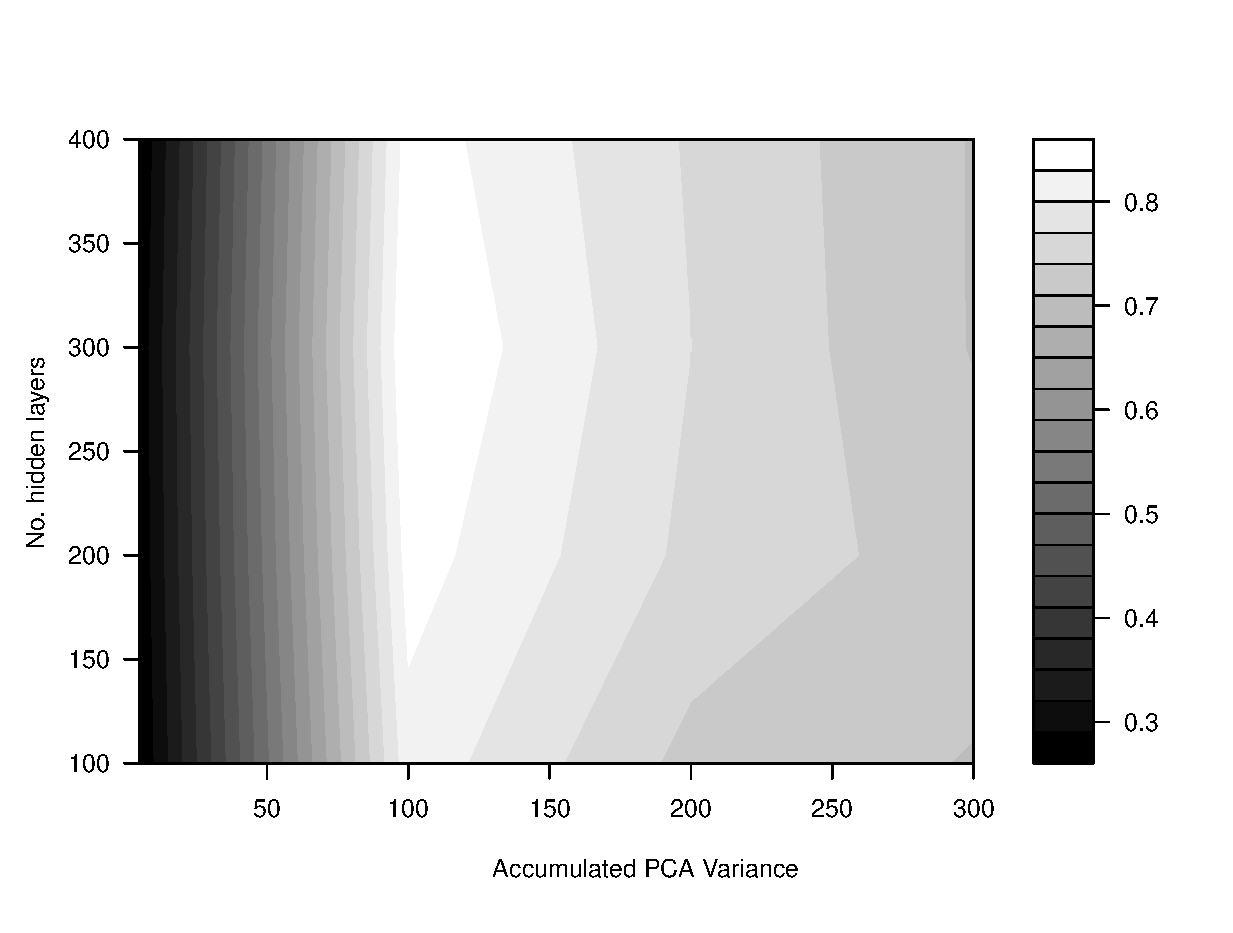
\includegraphics[width=\textwidth]{graphics/contour_nn_size_vs_pca}
    \caption[Success of ANN, PC vs HL]{Success of ANN when tested on G3M2 against everyone else's data.}
    \label{fig:contour_nn_size_vs_pca}
\end{figure}

The timing was measured in figure \ref{fig:contour_nn_both}.
The timing was split up into making the model and predicting the class.
The time it took to create the 10 models is shown in figure \ref{fig:contour_nn_size_vs_pca_time_model}.
% The time it took to predict all 4000 data points is shown in figure \ref{fig:contour_nn_size_vs_pca_time_predict}.
The biggest impact comes from number PC when building the model but the relationship is more linear when it comes to predicting.

\begin{figure}[h]
    \begin{subfigure}{0.49\textwidth}
    \centering
        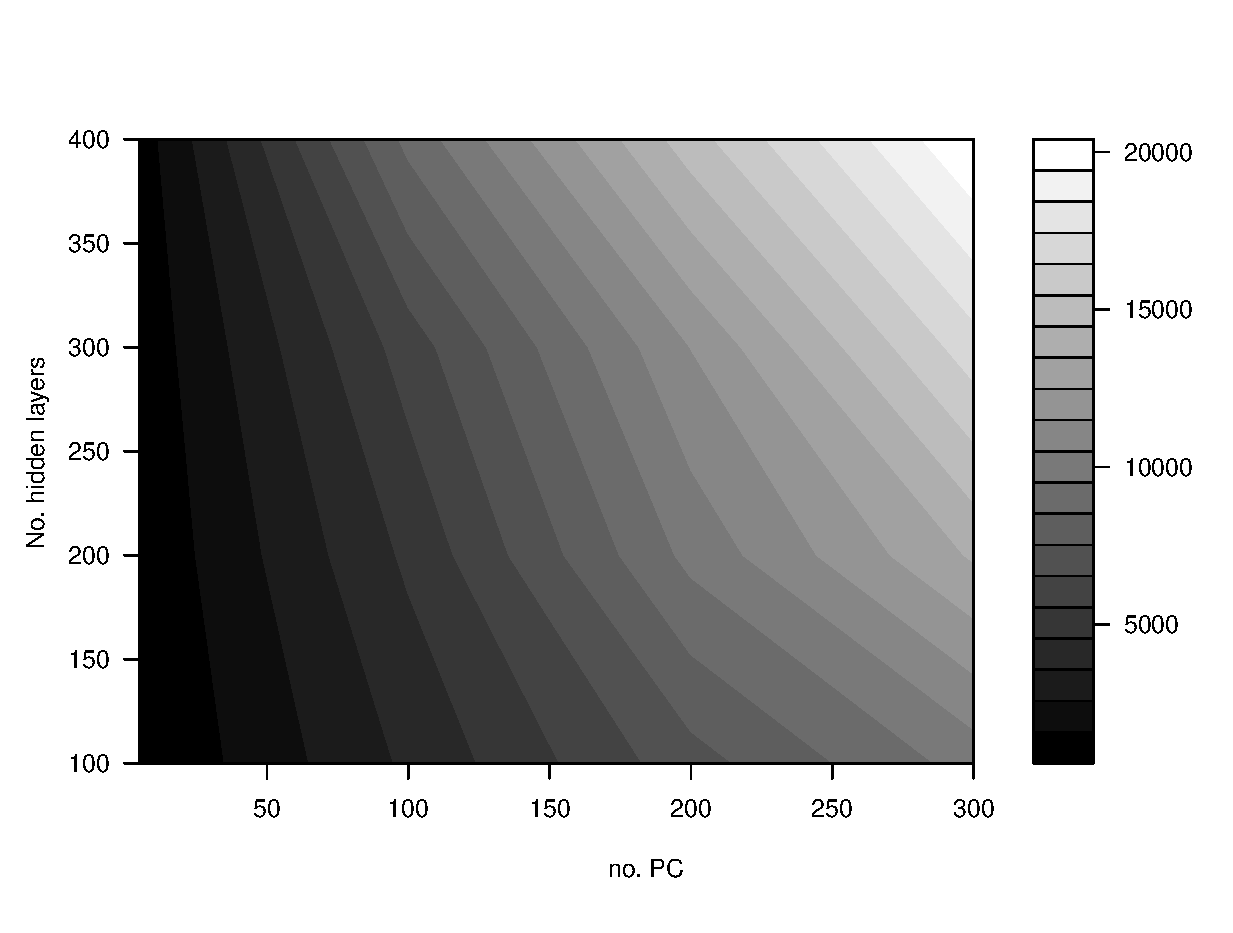
\includegraphics[width=\textwidth]{graphics/contour_nn_size_vs_pca_model}
        \caption{Time to build a ANN}
        \label{fig:contour_nn_size_vs_pca_time_model}
    \end{subfigure}
    \begin{subfigure}{0.49\textwidth}
        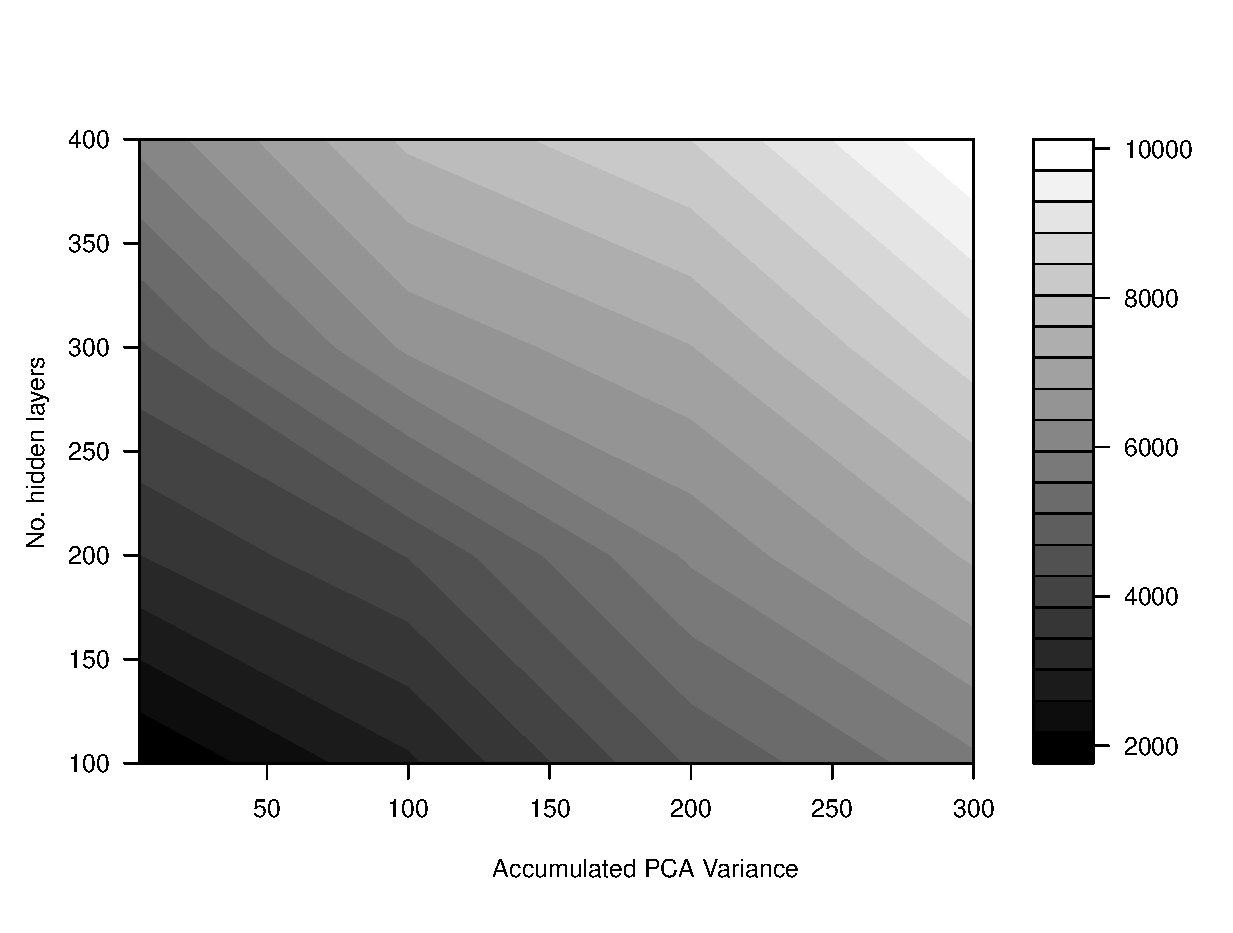
\includegraphics[width=\textwidth]{graphics/contour_nn_size_vs_pca_predict}
        \caption{Time of predicting using ANN}
        \label{fig:contour_nn_size_vs_pca_time_predict}
    \end{subfigure}
    \caption{Timing tested on G3M2 against everyone's data. The time is measured in seconds.}
    \label{fig:contour_nn_both}
\end{figure}

To view the impact of the train data size the timing and success was measured with a varying train set size.
The test is G3M2 tested against the rest of the students.
The data was normalized and the first 200 PC was used.
In all tests were 200 hidden layers in the ANN.
The Train size / digit refers to the number of samples per digit per person.
In figure \ref{fig:nn_timing_trainsize} is the timing and success plottet.
As expected is it shown that decreasing the train data will decrease the time it takes to build the model.
It is also shown that using more training digits does not increase the performance and thus this is a viable option.

\begin{figure}[h]
    \centering
    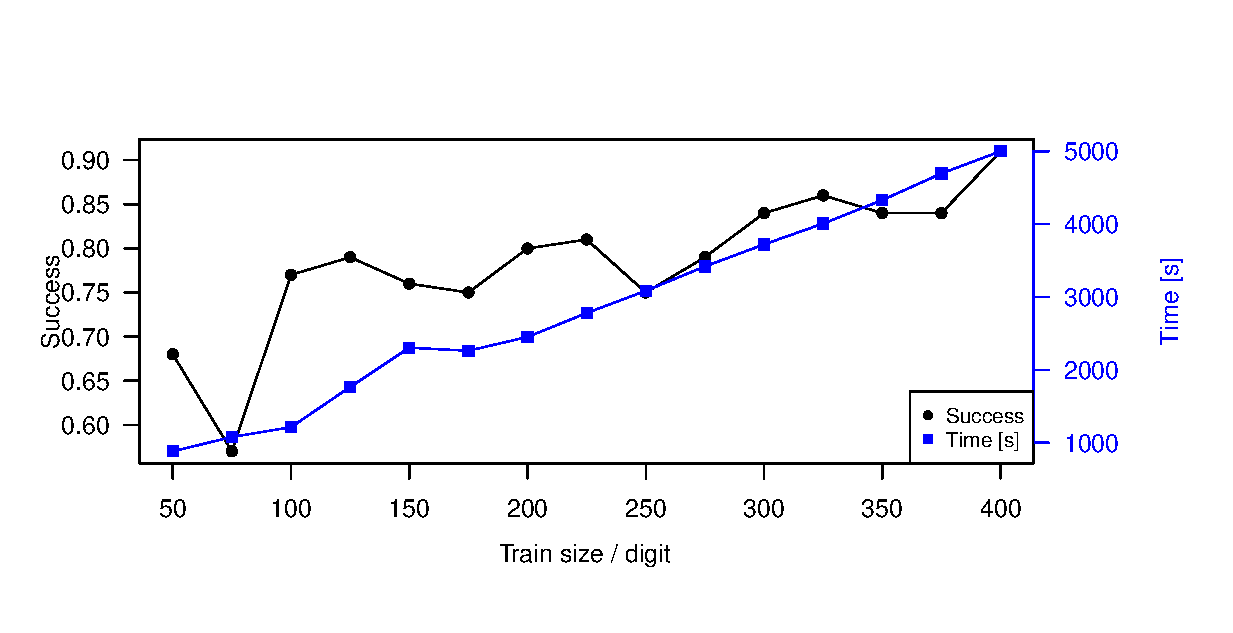
\includegraphics[width=\textwidth]{graphics/nn_timing_trainsize_200}
    \caption{Timing of building a ANN}
    \label{fig:nn_timing_trainsize}
\end{figure}


% \subsection{Support Vector Machines}
Support vector machines try to separate data in a multidimensional space into a subset of classes using a hyperplane.
Here the most common three kernels for SVMs will be considered.
These are, the Gaussian Radial Basis, the Polynomial and Linear kernel.

Below the optimum parameters for the Gaussian Radial Basis and the Polynomial kernel will be found.
As the Linear kernel does not have any parameters to change, it will be used directly in the test.

\subsubsection{Gaussian Radial Basis Kernel}
The Gaussian Radial Basis Kernel (RBF) function is given in equation \ref{eq:rbf}.

\begin{equation}
k(x,x') = \exp(-\sigma \|x - x'\|^2)
\label{eq:rbf}
\end{equation}

In figure \ref{fig:rbf} the result for the person independent test of G3M2 is shown when sigma goes from 0 to 6.
Only one person is used to decide the parameter in order to reduce processing time.

\begin{figure}[H]
\centering
\includegraphics[width = 0.9 \textwidth]{graphics/lineplot_svm_rbf}
\caption{Kernel success rate for different sigma values when using the Gaussian Radial Basis kernel.}
\label{fig:rbf}
\end{figure}

From figure \ref{fig:rbf} the optimum point can be found to be $\sigma = 2$.

\subsubsection{Polynomial Kernel}
The equation for the polynomial kernel is given in equation \ref{eq:poly}.

\begin{equation}
k(x,x') = (\text{scale} <x, x'> +\ \text{offset})^{\text{degree}}
\label{eq:poly}
\end{equation}

As seen in equation \ref{eq:poly}, then the polynomial function has 3 parameters to adjust.
These are the scale, offset and degree.
To simplify the selection of the optimum parameters, it was decided only to consider the scale and degree and use the default value for offset.
In figure \ref{fig:poly} the success for the person independent test of G3M2 is shown when the degree and scale goes from 1 to 4 and 0 to 0.08 respectively.

\begin{figure}[H]
\centering
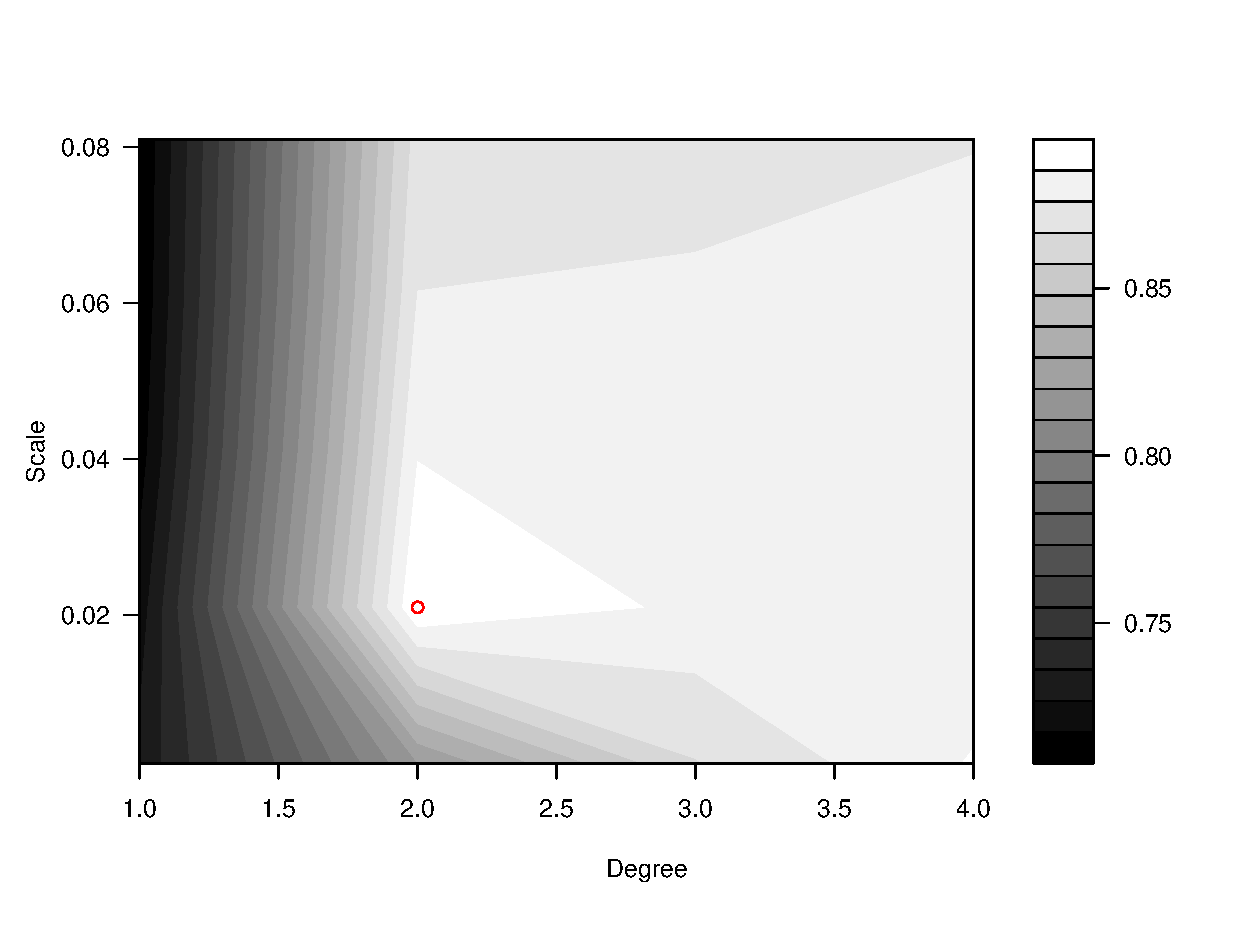
\includegraphics[width = 0.9 \textwidth]{graphics/contour_svm_poly}
\caption{Kernel success rate for different orders and scale values when using the poly kernel.
The red circle marks the point of which the success was found to be the maximum.}
\label{fig:poly}
\end{figure}

It was from figure \ref{fig:poly} found that the optimum scale and degree is 0.02 and 2 respectively when the default offset is used.


\subsubsection{Kernel Comparison}
The comparison of the three kernels can be seen in figure \ref{fig:comp_kernel}.
The Gaussian RBF was run with a sigma of 2 and the polynomial function a degree and scale of 2 and 0.02 respectively.


\begin{figure}[H]
\centering
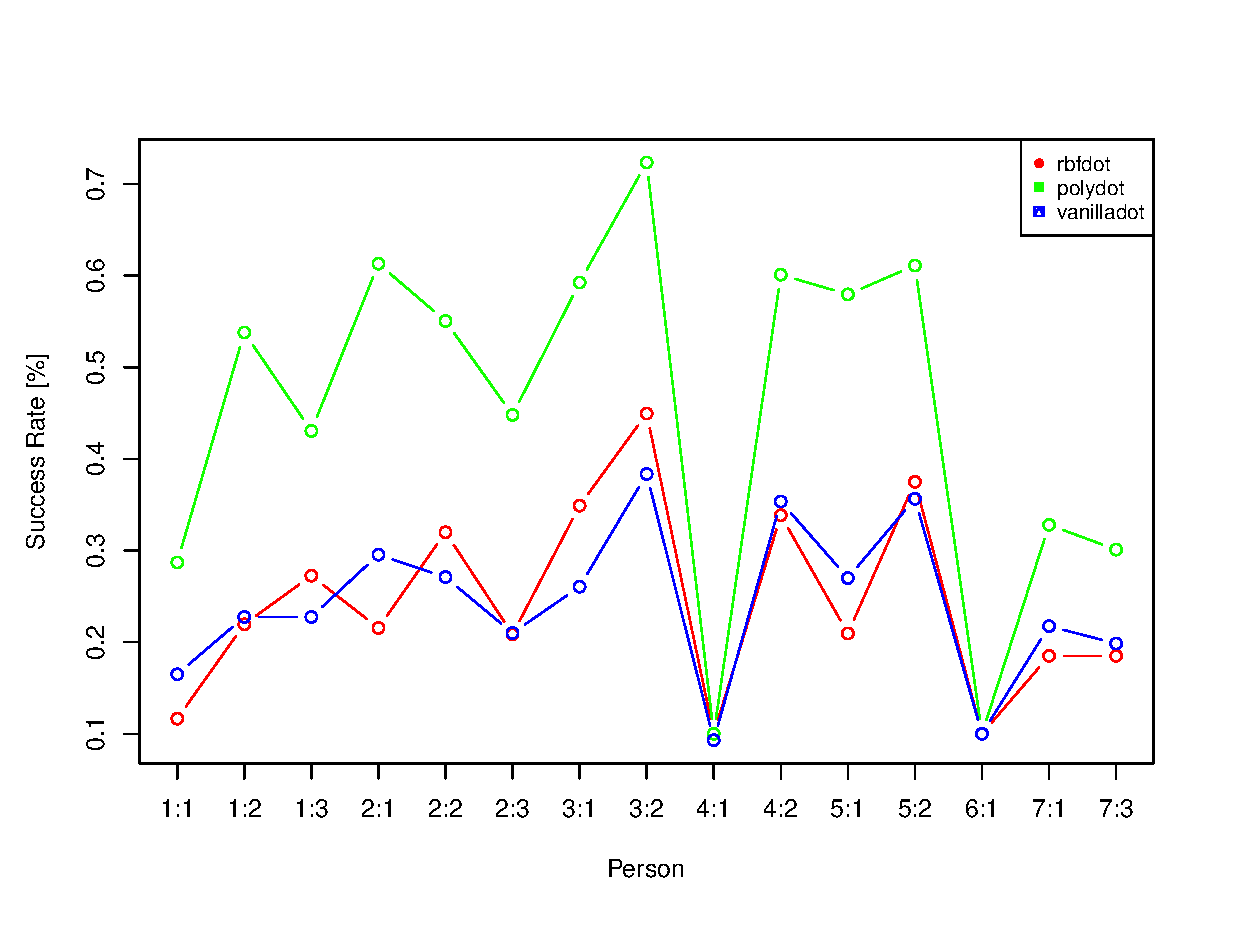
\includegraphics[width = \textwidth]{graphics/svm_kernel_comp}
\caption{Comparison of 15 independent datasets and the SVM kernel used. The mean success rate of the datasets are shown in table \ref{tab:mean_succes_kernel}.}
\label{fig:comp_kernel}
\end{figure}

%"mean rbf: 0.242933333333333
%"mean poly: "       "0.453566666666667"
%"mean vanilla: "    "0.241966666666667"

\begin{table}[H]
\centering
\begin{tabular}{|l|c|}
\hline
Kernel & Mean Success\\ \hline
RBF & 24.29 \% \\ \hline
Polynomial & 45.36 \% \\ \hline
Vanilla & 24.20 \% \\ \hline
\end{tabular}
\caption{Mean success rate of figure \ref{fig:comp_kernel}.}
\label{tab:mean_succes_kernel}
\end{table}


As seen on figure \ref{fig:comp_kernel} and in table \ref{tab:mean_succes_kernel}, then the polynomial kernel is performing almost twice as good as the two other kernels for this classification problem.
%The two sudden drops in success in figure \ref{fig:comp_kernel} at 4:1 and 6:1 are surprising because of their success of all three kernels being approximately equal, but it is not possible for us to explain why this is the case.





\end{document}